% Use only LaTeX2e, calling the article.cls class and 12-point type.

\documentclass[12pt]{article}

% -----------------------------------------------------
\usepackage{parskip}
\usepackage{float}
\usepackage{pdflscape}
\usepackage{datetime}
\usepackage{amsmath}
\usepackage{amssymb}
\usepackage[flushleft]{threeparttable}
% \usepackage{dcolumn}
\usepackage{siunitx} % align columns with dots and commas
\usepackage{lscape}
\setlength\parindent{0pt}
\usepackage{xcolor}
\usepackage{appendix}
\usepackage{graphicx}
\usepackage{hyperref}
\usepackage[capposition=top]{floatrow}
\graphicspath{{figures/}} %Setting the graphicspath
\usepackage{subcaption}
\renewcommand{\thesubfigure}{\Alph{subfigure}}
\usepackage[export]{adjustbox}
\usepackage{rotating}
\usepackage{booktabs}
\usepackage{subfig}
\captionsetup[subfigure]{labelfont = {bf, small}, font = small}

% upper left corner
% \captionsetup[subfigure]{labelfont = bf, font = small, singlelinecheck=false}

% -----------------------------------------------------

% Users of the {thebibliography} environment or BibTeX should use the
% scicite.sty package, downloadable from *Science* at
% www.sciencemag.org/about/authors/prep/TeX_help/ .
% This package should properly format in-text
% reference calls and reference-list numbers.

\usepackage{scicite}

% Use times if you have the font installed; otherwise, comment out the
% following line.

\usepackage{times}

% The preamble here sets up a lot of new/revised commands and
% environments.  It's annoying, but please do *not* try to strip these
% out into a separate .sty file (which could lead to the loss of some
% information when we convert the file to other formats).  Instead, keep
% them in the preamble of your main LaTeX source file.


% The following parameters seem to provide a reasonable page setup.

\topmargin 0.0cm
\oddsidemargin 0.2cm
\textwidth 16cm 
\textheight 21cm
\footskip 1.0cm


%The next command sets up an environment for the abstract to your paper.

\newenvironment{sciabstract}{%
\begin{quote} \bf}
{\end{quote}}


% If your reference list includes text notes as well as references,
% include the following line; otherwise, comment it out.

\renewcommand\refname{References and Notes}

% The following lines set up an environment for the last note in the
% reference list, which commonly includes acknowledgments of funding,
% help, etc.  It's intended for users of BibTeX or the {thebibliography}
% environment.  Users who are hand-coding their references at the end
% using a list environment such as {enumerate} can simply add another
% item at the end, and it will be numbered automatically.

\newcounter{lastnote}
\newenvironment{scilastnote}{%
\setcounter{lastnote}{\value{enumiv}}%
\addtocounter{lastnote}{+1}%
\begin{list}%
{\arabic{lastnote}.}
{\setlength{\leftmargin}{.22in}}
{\setlength{\labelsep}{.5em}}}
{\end{list}}


% Include your paper's title here

\title{Can Social and Traditional Media Campaigns Empower Women Subjected to Gender-Based Amid COVID-19?} 

% Place the author information here.  Please hand-code the contact
% information and notecalls; do *not* use \footnote commands.  Let the
% author contact information appear immediately below the author names
% as shown.  We would also prefer that you don't change the type-size
% settings shown here.

\author
{John Smith,$^{1\ast}$ Jane Doe,$^{1}$ Joe Scientist$^{2}$\\
\\
\normalsize{$^{1}$Department of , University of Wherever,}\\
\normalsize{An Unknown Address, Wherever, ST 00000, USA}\\
\normalsize{$^{2}$Another Unknown Address, Palookaville, ST 99999, USA}\\
\\
\normalsize{$^\ast$To whom correspondence should be addressed; E-mail:  jsmith@wherever.edu.}
}

% Include the date command, but leave its argument blank.

\date{}



%%%%%%%%%%%%%%%%% END OF PREAMBLE %%%%%%%%%%%%%%%%



\begin{document} 

% Double-space the manuscript.

\baselineskip24pt

% Make the title.

\maketitle 



% Place your abstract within the special {sciabstract} environment.

\begin{sciabstract}
Women's exposure to gender-based violence (GBV) may be especially acute amid COVID-19, which has led to a notable increase in reported violence, particularly in the  Global South. Building on recent studies on the role of edutainment and community-level interventions in combating GBV, we partnered with an Egyptian women’s rights non-governmental organization to evaluate a randomized intervention delivered amid COVID-19 via social (Facebook and WhatsApp) and traditional (TV) media that are widely used in the Egyptian context. Our findings show that overall the intervention led to increased knowledge and use of resources available for women subjected to GBV, while it did not affect exposure to GBV and attitudes toward gender and marital equality, and sexual violence. WhatsApp was a more effective way for respondents to consume the treatment information than Facebook, but there are no statistical differences in knowledge and use of resources between WhatsApp and TV dissemination.
\end{sciabstract}



% In setting up this template for *Science* papers, we've used both
% the \section* command and the \paragraph* command for topical
% divisions.  Which you use will of course depend on the type of paper
% you're writing.  Review Articles tend to have displayed headings, for
% which \section* is more appropriate; Research Articles, when they have
% formal topical divisions at all, tend to signal them with bold text
% that runs into the paragraph, for which \paragraph* is the right
% choice.  Either way, use the asterisk (*) modifier, as shown, to
% suppress numbering.

%\section*{Introduction}
%\section*{Sections with brief subheadings}
% Introduction (check how much papers advance the results)
% 
% Context and Intervention
% To Appendix: Recruitment, and Treatment Assignment should mostly go there.
% 
%\section*{Conclusion}
% Materials and Methods should be included in supplementary materials


COVID-19 has heightened the extent and risk of gender-based violence (GBV) and intimate-partner violence (IPV), particularly in the Global South. \textcolor{blue}{\bf Manuel: can you please turn all these footnotes into references in the .bib file and cite the appropriately.}\footnote{Rivera et. al, \say{What does coronavirus mean for women?}, United Nations Development Programme, July 13, 2020, \href{https://www.undp.org/content/undp/en/home/blog/2020/what-does-coronavirus-mean-for-women.html}{Link}; %\footnote{
\say{Gendered Impact of Covid-19 Outbreaks in Development and Humanitarian Settings,} \textit{CARE}, March 16, 2020, \href{https://care.org/wp-content/uploads/2020/07/gendered_implications_of_covid-19_-_full_paper.pdf}{Link}.} The policies implemented to help contain the spread of COVID-19 have often included significant mobility restrictions. These policies had imposed a significant toll on the economy adding significant economic stress to the existing social stress and reducing women economic empowerment.\footnote{\href{https://advances.sciencemag.org/content/7/6/eabe0997}{Link}}\textcolor{blue}{\bf Manuel: can you please add footnote to citations and cite it properly?} 
Combined with existing social norms toward women, these policies ultimately increased the extent and risk of GBV and IPV of women across the globe.





\section*{Formatting Citations}

Citations can be handled in one of three ways.  The most
straightforward (albeit labor-intensive) would be to hardwire your
citations into your \LaTeX\ source, as you would if you were using an
ordinary word processor.  Thus, your code might look something like
this:


\noindent Compiled, the last two lines of the code above, of course, would give notecalls in {\it Science\/} style:

\begin{quote}
\ldots thermal metamorphism, and aqueous alteration ({\it 1, 2, 5--7\/}).
\end{quote}

Under the same logic, the author could set up his or her reference list as a simple enumeration,

\begin{quote}
\begin{verbatim}
{\bf References and Notes}

\begin{enumerate}
\item G. Gamow, {\it The Constitution of Atomic Nuclei
and Radioactivity\/} (Oxford Univ. Press, New York, 1931).
\item W. Heisenberg and W. Pauli, {\it Zeitschr.\ f.\ 
Physik\/} {\bf 56}, 1 (1929).
\end{enumerate}
\end{verbatim}
\end{quote}

\noindent yielding

\begin{quote}
{\bf References and Notes}

\begin{enumerate}
\item G. Gamow, {\it The Constitution of Atomic Nuclei and
Radioactivity\/} (Oxford Univ. Press, New York, 1931).
\item W. Heisenberg and W. Pauli, {\it Zeitschr.\ f.\ Physik} {\bf 56},
1 (1929).
\end{enumerate}
\end{quote}

That's not a solution that's likely to appeal to everyone, however ---
especially not to users of B{\small{IB}}\TeX\ \cite{inclme}.  If you
are a B{\small{IB}}\TeX\ user, we suggest that you use the
\texttt{Science.bst} bibliography style file and the
\texttt{scicite.sty} package, both of which we are downloadable from our author help site
(http://www.sciencemag.org/about/authors/prep/TeX\_help/).  You can also
generate your reference lists by using the list environment
\texttt{\{thebibliography\}} at the end of your source document; here
again, you may find the \texttt{scicite.sty} file useful.

Whether you use B{\small{IB}}\TeX\ or \texttt{\{thebibliography\}}, be
very careful about how you set up your in-text reference calls and
notecalls.  In particular, observe the following requirements:

\begin{enumerate}
\item Please follow the style for references outlined at our author
  help site and embodied in recent issues of {\it Science}.  Each
  citation number should refer to a single reference; please do not
  concatenate several references under a single number.
\item Please cite your references and notes in text {\it only\/} using
  the standard \LaTeX\ \verb+\cite+ command, not another command
  driven by outside macros.
\item Please separate multiple citations within a single \verb+\cite+
  command using commas only; there should be {\it no space\/}
  between reference keynames.  That is, if you are citing two
  papers whose bibliography keys are \texttt{keyname1} and
  \texttt{keyname2}, the in-text cite should read
  \verb+\cite{keyname1,keyname2}+, {\it not\/}
  \verb+\cite{keyname1, keyname2}+.
\end{enumerate}

\noindent Failure to follow these guidelines could lead
to the omission of the references in an accepted paper when the source
file is translated to Word97 via HTML.

\section*{Handling Math, Tables, and Figures}

Following are a few things to keep in mind in coding equations,
tables, and figures for submission to {\it Science}.

\paragraph*{In-line math.}  The utility that we use for converting
from \LaTeX\ to HTML handles in-line math relatively well.  It is best
to avoid using built-up fractions in in-line equations, and going for
the more boring ``slash'' presentation whenever possible --- that is,
for \verb+$a/b$+ (which comes out as $a/b$) rather than
\verb+$\frac{a}{b}$+ (which compiles as $\frac{a}{b}$).  Likewise,
HTML isn't tooled to handle certain overaccented special characters
in-line; for $\hat{\alpha}$ (coded \verb+$\hat{\alpha}$+), for
example, the HTML translation code will return [\^{}$(\alpha)$].
Don't drive yourself crazy --- but if it's possible to avoid such
constructs, please do so.  Please do not code arrays or matrices as
in-line math; display them instead.  And please keep your coding as
\TeX-y as possible --- avoid using specialized math macro packages
like \texttt{amstex.sty}.

\paragraph*{Displayed math.} Our HTML converter sets up \TeX\
displayed equations using nested HTML tables.  That works well for an
HTML presentation, but Word97 chokes when it comes across a nested
table in an HTML file.  We surmount that problem by simply cutting the
displayed equations out of the HTML before it's imported into Word97,
and then replacing them in the Word document using either images or
equations generated by a Word equation editor.  Strictly speaking,
this procedure doesn't bear on how you should prepare your manuscript
--- although, for reasons best consigned to a note \cite{nattex}, we'd
prefer that you use native \TeX\ commands within displayed-math
environments, rather than \LaTeX\ sub-environments.

\paragraph*{Tables.}  The HTML converter that we use seems to handle
reasonably well simple tables generated using the \LaTeX\
\texttt{\{tabular\}} environment.  For very complicated tables, you
may want to consider generating them in a word processing program and
including them as a separate file.

\paragraph*{Figures.}  Figure callouts within the text should not be
in the form of \LaTeX\ references, but should simply be typed in ---
that is, \verb+(Fig. 1)+ rather than \verb+\ref{fig1}+.  For the
figures themselves, treatment can differ depending on whether the
manuscript is an initial submission or a final revision for acceptance
and publication.  For an initial submission and review copy, you can
use the \LaTeX\ \verb+{figure}+ environment and the
\verb+\includegraphics+ command to include your PostScript figures at
the end of the compiled PostScript file.  For the final revision,
however, the \verb+{figure}+ environment should {\it not\/} be used;
instead, the figure captions themselves should be typed in as regular
text at the end of the source file (an example is included here), and
the figures should be uploaded separately according to the Art
Department's instructions.


\section*{What to Send In}

What you should send to {\it Science\/} will depend on the stage your manuscript is in:

\begin{itemize}
\item {\bf Important:} If you're sending in the initial submission of
  your manuscript (that is, the copy for evaluation and peer review),
  please send in {\it only\/} a PostScript or PDF version of the
  compiled file (including figures).  Please do not send in the \TeX\ 
  source, \texttt{.sty}, \texttt{.bbl}, or other associated files with
  your initial submission.  (For more information, please see the
  instructions at our Web submission site,
  http://www.submit2science.org/ .)
\item When the time comes for you to send in your revised final
  manuscript (i.e., after peer review), we require that you include
  all source files and generated files in your upload.  Thus, if the
  name of your main source document is \texttt{ltxfile.tex}, you
  need to include:
\begin{itemize}
\item \texttt{ltxfile.tex}.
\item \texttt{ltxfile.aux}, the auxilliary file generated by the
  compilation.
\item A PostScript file (compiled using \texttt{dvips} or some other
  driver) of the \texttt{.dvi} file generated from
  \texttt{ltxfile.tex}, or a PDF file distilled from that
  PostScript.  You do not need to include the actual \texttt{.dvi}
  file in your upload.
\item From B{\small{IB}}\TeX\ users, your bibliography (\texttt{.bib})
  file, {\it and\/} the generated file \texttt{ltxfile.bbl} created
  when you run B{\small{IB}}\TeX.
\item Any additional \texttt{.sty} and \texttt{.bst} files called by
  the source code (though, for reasons noted earlier, we {\it
    strongly\/} discourage the use of such files beyond those
  mentioned in this document).
\end{itemize}
\end{itemize}

% Your references go at the end of the main text, and before the
% figures.  For this document we've used BibTeX, the .bib file
% scibib.bib, and the .bst file Science.bst.  The package scicite.sty
% was included to format the reference numbers according to *Science*
% style.


\bibliography{scibib}

\bibliographystyle{Science}



% Following is a new environment, {scilastnote}, that's defined in the
% preamble and that allows authors to add a reference at the end of the
% list that's not signaled in the text; such references are used in
% *Science* for acknowledgments of funding, help, etc.

\begin{scilastnote}
\item We've included in the template file \texttt{scifile.tex} a new
environment, \texttt{\{scilastnote\}}, that generates a numbered final
citation without a corresponding signal in the text.  This environment
can be used to generate a final numbered reference containing
acknowledgments, sources of funding, and the like, per {\it Science\/}
style.  Along those lines, we'd like to thank readers of this document
for their attention, and invite them to address any questions to
Stewart Wills, at swills@aaas.org.
\end{scilastnote}




% For your review copy (i.e., the file you initially send in for
% evaluation), you can use the {figure} environment and the
% \includegraphics command to stream your figures into the text, placing
% all figures at the end.  For the final, revised manuscript for
% acceptance and production, however, PostScript or other graphics
% should not be streamed into your compliled file.  Instead, set
% captions as simple paragraphs (with a \noindent tag), setting them
% off from the rest of the text with a \clearpage as shown  below, and
% submit figures as separate files according to the Art Department's
% instructions.


\clearpage

\noindent {\bf Fig. 1.} Please do not use figure environments to set
up your figures in the final (post-peer-review) draft, do not include graphics in your
source code, and do not cite figures in the text using \LaTeX\
\verb+\ref+ commands.  Instead, simply refer to the figure numbers in
the text per {\it Science\/} style, and include the list of captions at
the end of the document, coded as ordinary paragraphs as shown in the
\texttt{scifile.tex} template file.  Your actual figure files should
be submitted separately.


\setcounter{figure}{0}
\renewcommand{\figurename}{Fig.}
\renewcommand{\thefigure}{\arabic{figure}}


\begin{figure}[H]
\caption{Comparison of demographics between Arab Barometer and experimental sample respondents}
  \begin{subfigure}[b]{0.48\linewidth}
    \centering
    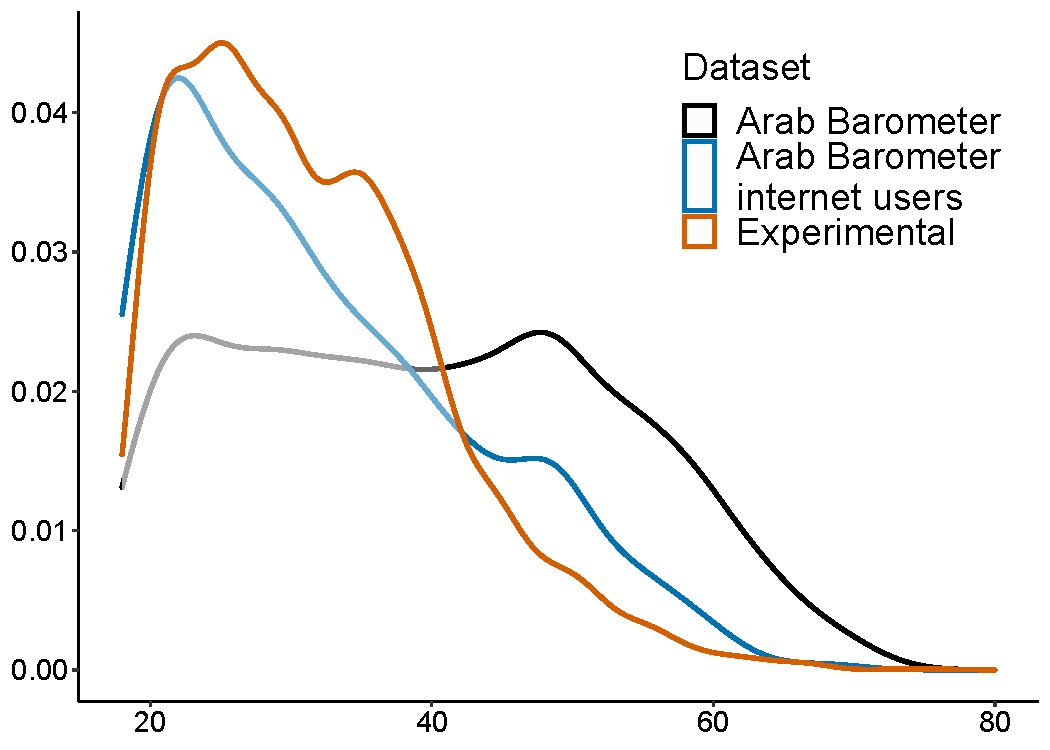
\includegraphics[height=6cm,width=8cm\linewidth]{Figures/AB/white/age.pdf} 
    \caption{Age} 
    \label{} 
  \end{subfigure} 
  \hspace{\fill}  
  \begin{subfigure}[b]{0.48\linewidth}
    \centering
    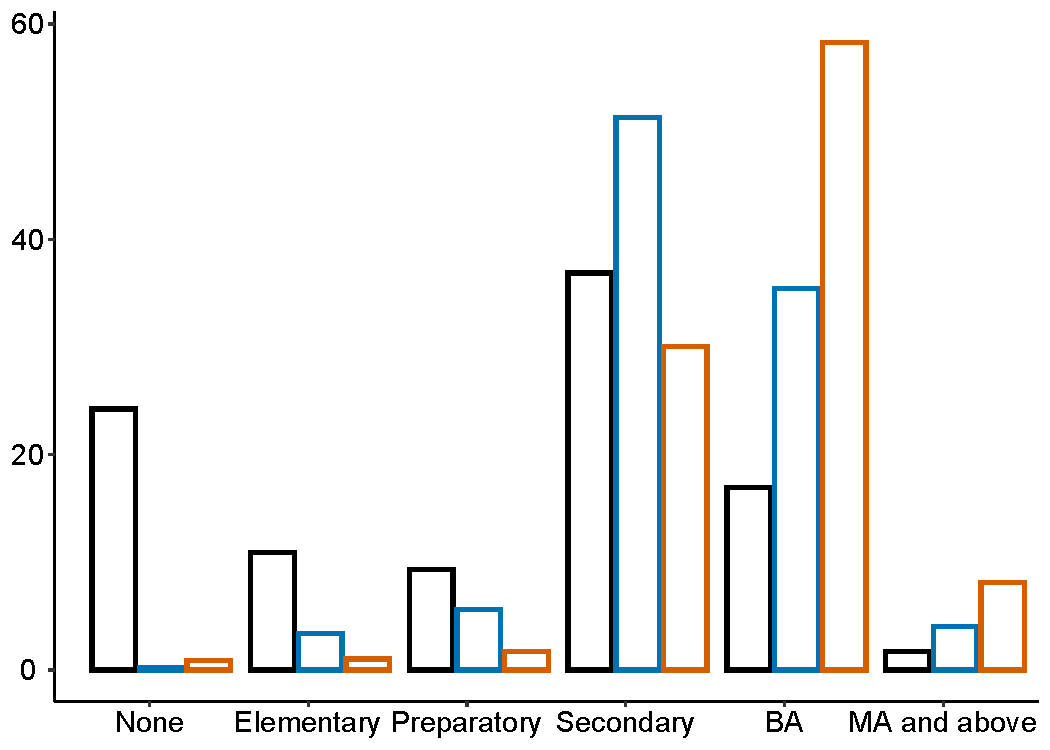
\includegraphics[height=6cm,width=8cm\linewidth]{Figures/AB/white/educ.pdf}
    \caption{Education level} 
    \label{} 
  \end{subfigure} 
  \begin{subfigure}[b]{0.48\linewidth}
    \centering
    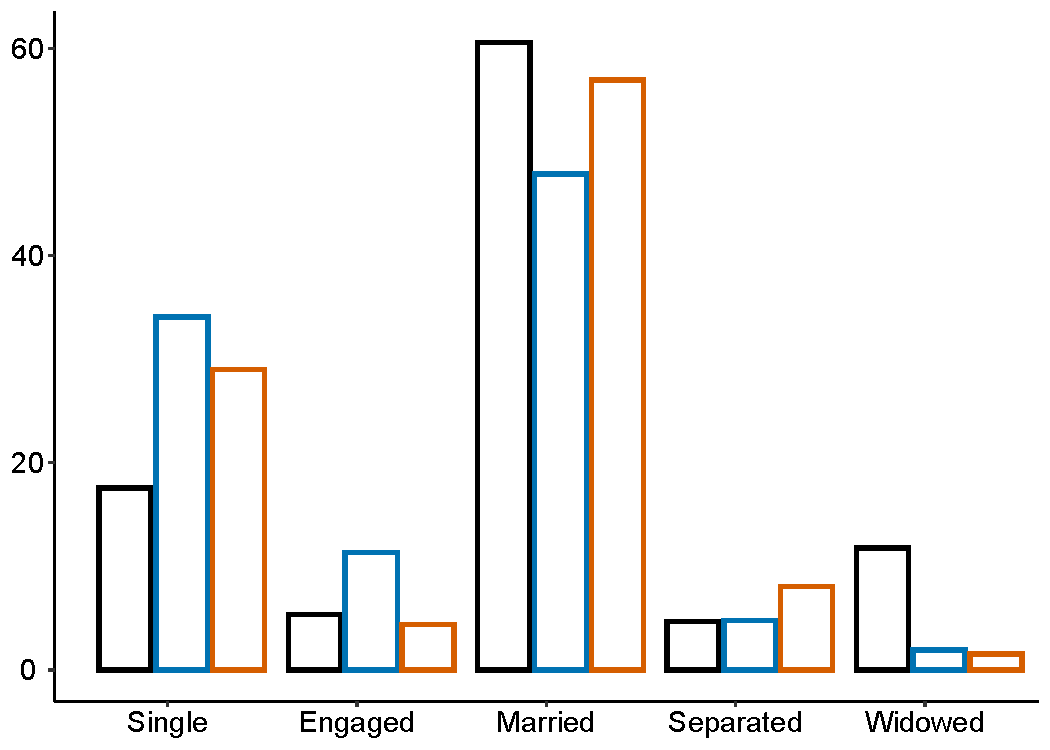
\includegraphics[height=6cm,width=8cm\linewidth]{Figures/AB/white/married.pdf} 
    \caption{Social status} 
    \label{} 
  \end{subfigure} 
  \hspace{\fill}
  \begin{subfigure}[b]{0.48\linewidth}
    \centering
    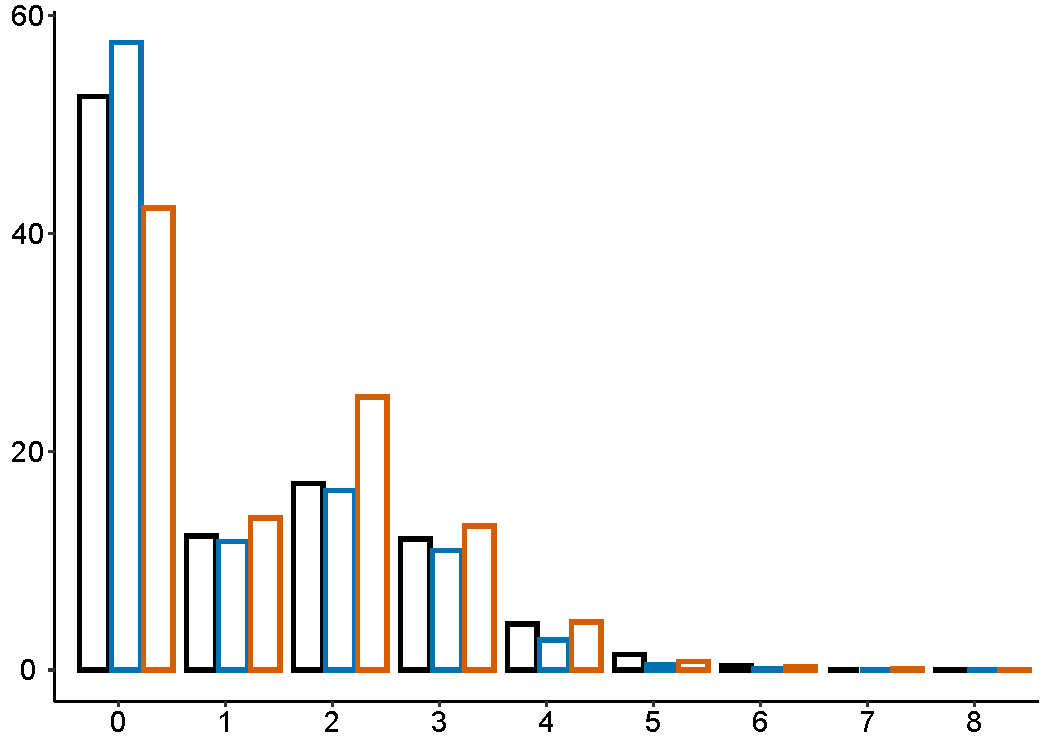
\includegraphics[height=6cm,width=8cm\linewidth]{Figures/AB/white/child.pdf} 
    \caption{Number of children} 
    \label{} 
  \end{subfigure} 

  \begin{subfigure}[b]{0.48\linewidth}
    \centering
    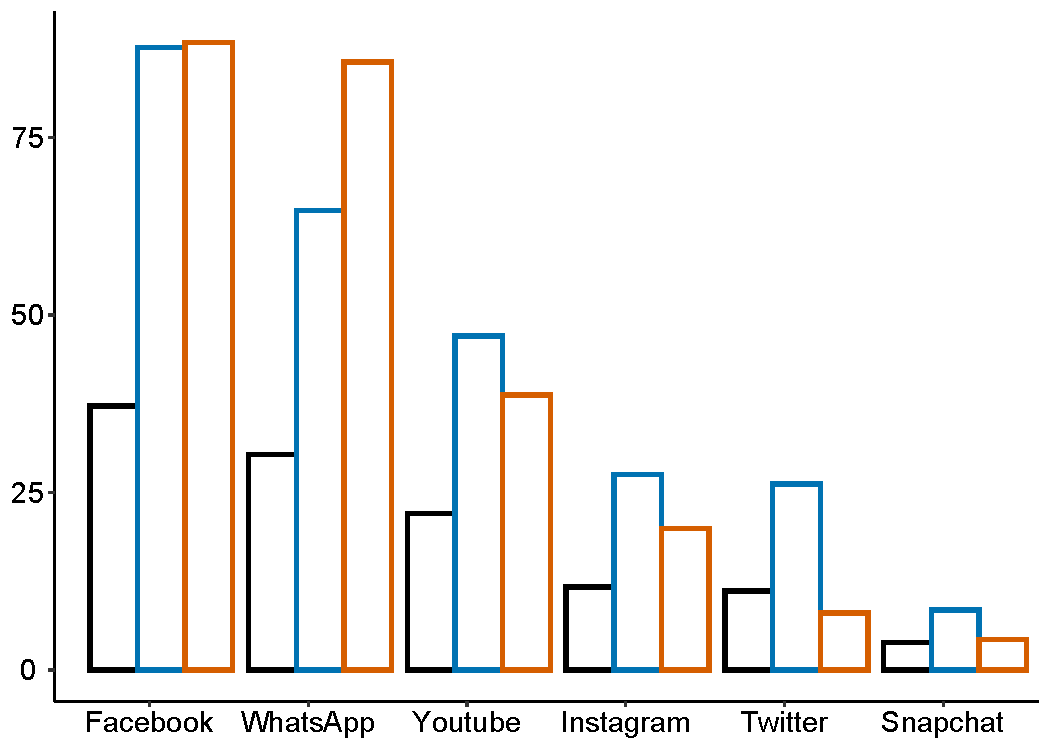
\includegraphics[height=6cm,width=8cm\linewidth]{Figures/AB/white/which_sm.pdf} 
    \caption{Social media use} 
    \label{} 
  \end{subfigure}
  \hspace{\fill}
  \begin{subfigure}[b]{0.48\linewidth}
    \centering
    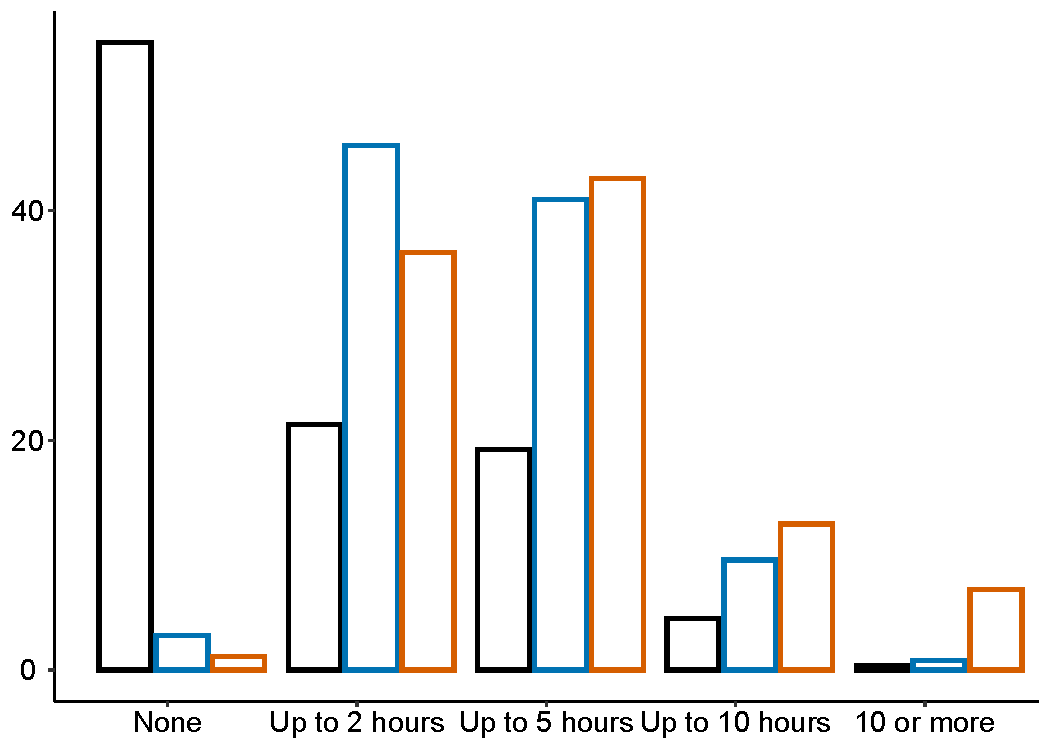
\includegraphics[height=6cm,width=8cm\linewidth]{Figures/AB/white/hours_sm.pdf} 
    \caption{Weekly hours spent on social media} 
    \label{} 
  \end{subfigure} 

\end{figure}


\begin{figure}[H]
    \centering
    \caption{Treatment effects on TV show consumption, Facebook and WhatsApp treatment consumption, and knowledge of resources delivered in treatment}
    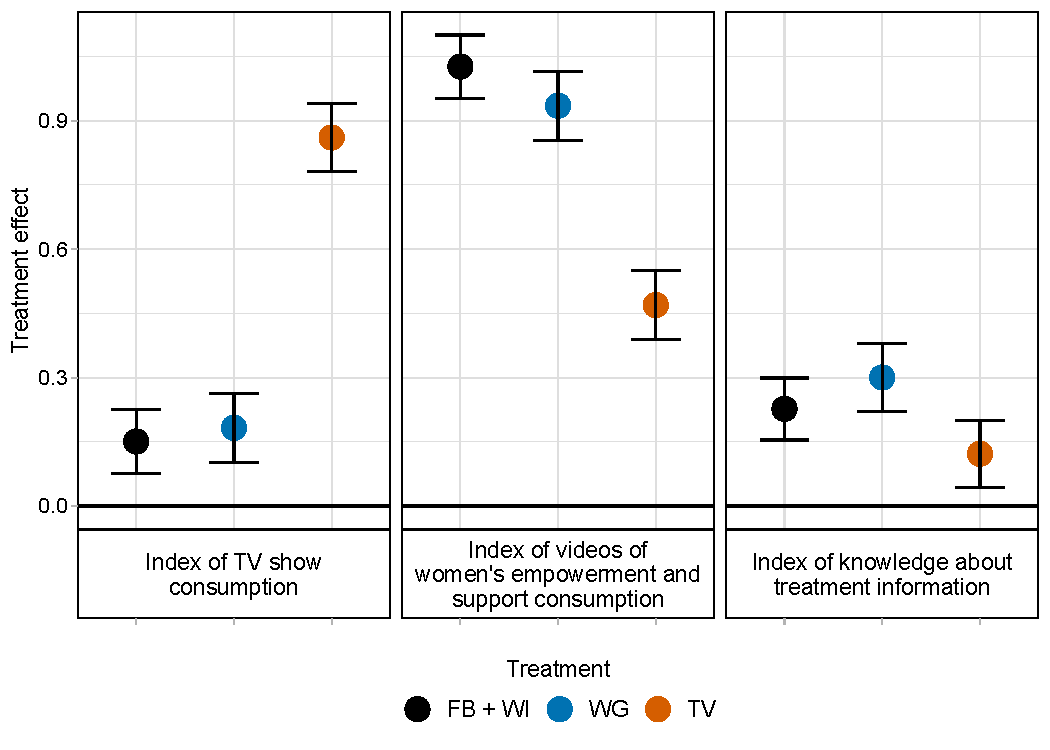
\includegraphics[width=12cm, height=9cm\textwidth]{Figures/RF-FS/Figure2.pdf}
    \captionsetup{width=.75\linewidth}
    \caption*{\footnotesize \textit{Notes:} The estimates and $95$\% confidence intervals in each box are from separate WGLS regressions where the weights are in the inverse probability of treatment assignment. The labels are the corresponding dependent variables regressed on treatment indicators (FB $+$ WI $=$ Facebook or WhatsApp individual message, WG $=$ WhatsApp group message, TV $=$ TV show reminder), relevant baseline controls and randomization block fixed effects. The outcomes included in the index of TV show consumption are in Table S$13$. The outcomes included in the index of videos of women’s empowerment and support are in Table S$14$. The outcomes included in the index of knowledge about treatment information are in Table S$15$.}
\end{figure}



\begin{figure}[H]
    \centering
    \caption{Treatment effects on attitudes toward gender and marital equality, and sexual violence}
    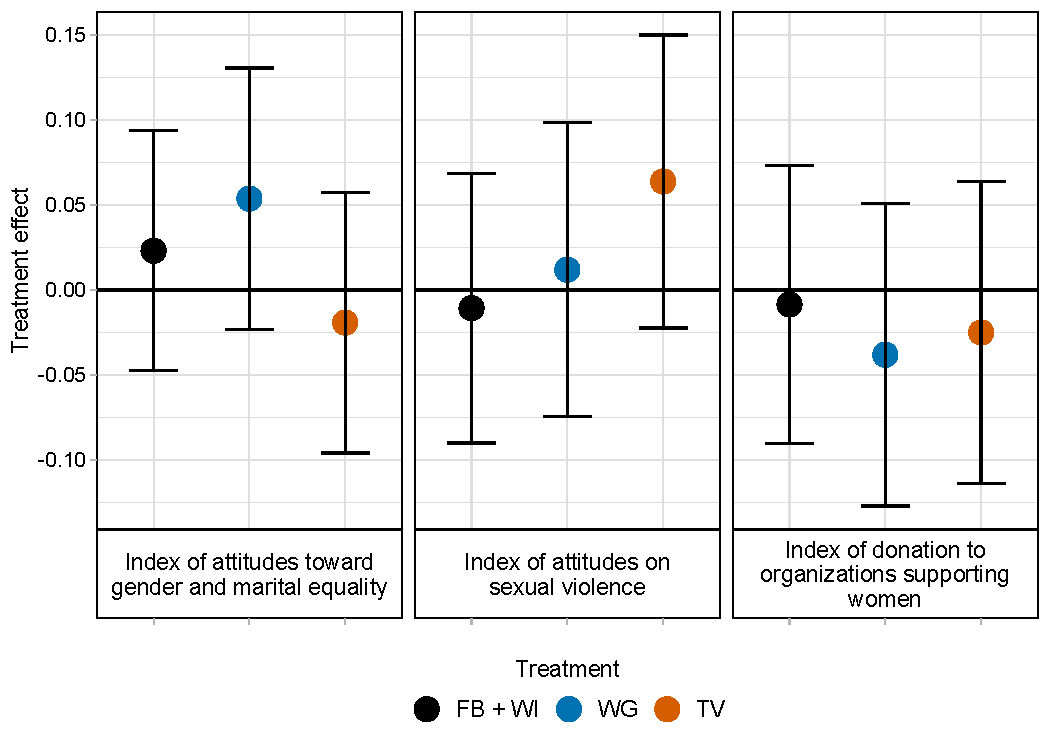
\includegraphics[width=12cm, height=9cm\textwidth]{Figures/RF-FS/Figure3.pdf}
        \captionsetup{width=.75\linewidth}
    \caption*{\footnotesize \textit{Notes:} The estimates and $95$\% confidence intervals in each box are from separate WGLS regressions where the weights are in the inverse probability of treatment assignment. The labels are the corresponding dependent variables regressed on treatment indicators (FB $+$ WI $=$ Facebook or WhatsApp individual message, WG $=$ WhatsApp group message, TV $=$ TV show reminder), relevant baseline controls and randomization block fixed effects. The outcomes included in the index of attitudes toward gender and marital equality are in Table S16. The outcomes included in the index of attitudes on sexual violence are in Table S$17$. The outcomes included in the index of donation to organizations supporting women are in Table S$18$.}
\end{figure}


\begin{figure}[H]
    \centering
    \caption{Treatment effects on violence experienced during COVID-19, hypothetical and recent use of online resources or contact with an organization when responding to domestic or sexual violence}
    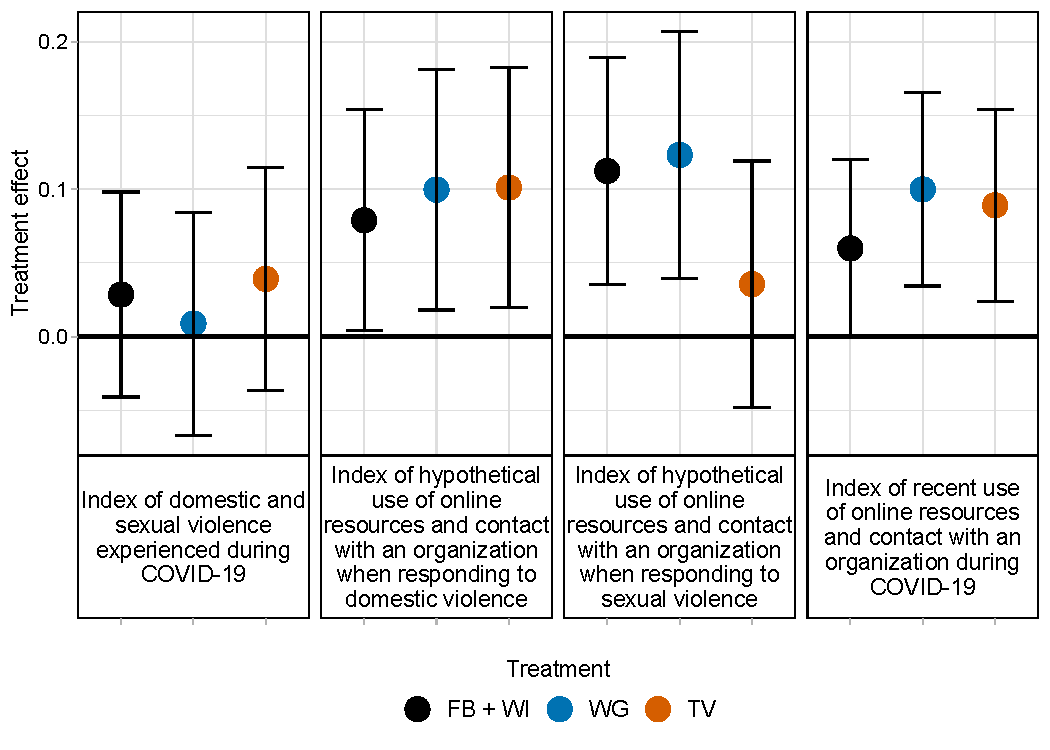
\includegraphics[width=12cm, height=9cm\textwidth]{Figures/RF-FS/Figure4.pdf}
    \captionsetup{width=.75\linewidth}
    \caption*{\footnotesize \textit{Notes:} The estimates and $95$\% confidence intervals in each box are from separate WGLS regressions where the weights are in the inverse probability of treatment assignment. The labels are the corresponding dependent variables regressed on treatment indicators (FB $+$ WI $=$ Facebook or WhatsApp individual message, WG $=$ WhatsApp group message, TV $=$ TV show reminder), relevant baseline controls and randomization block fixed effects. The outcomes included in the index of domestic and sexual violence experienced during COVID-19 are in Table S$19$. The outcomes included in the index of hypothetical use of online resources and contact with an organization when responding to domestic violence are in Table S20. The outcomes included in the index of hypothetical use of online resources and contact with an organization when responding to sexual violence are in Table S$21$. The outcomes included in the index of recent use of online resources and contact with an organization during COVID-19 are those in Table S$22$.}
\end{figure}



\begin{figure}[H]
    \centering
    \caption{Treatment effects on women’s future outlook toward gender and marital equality}
    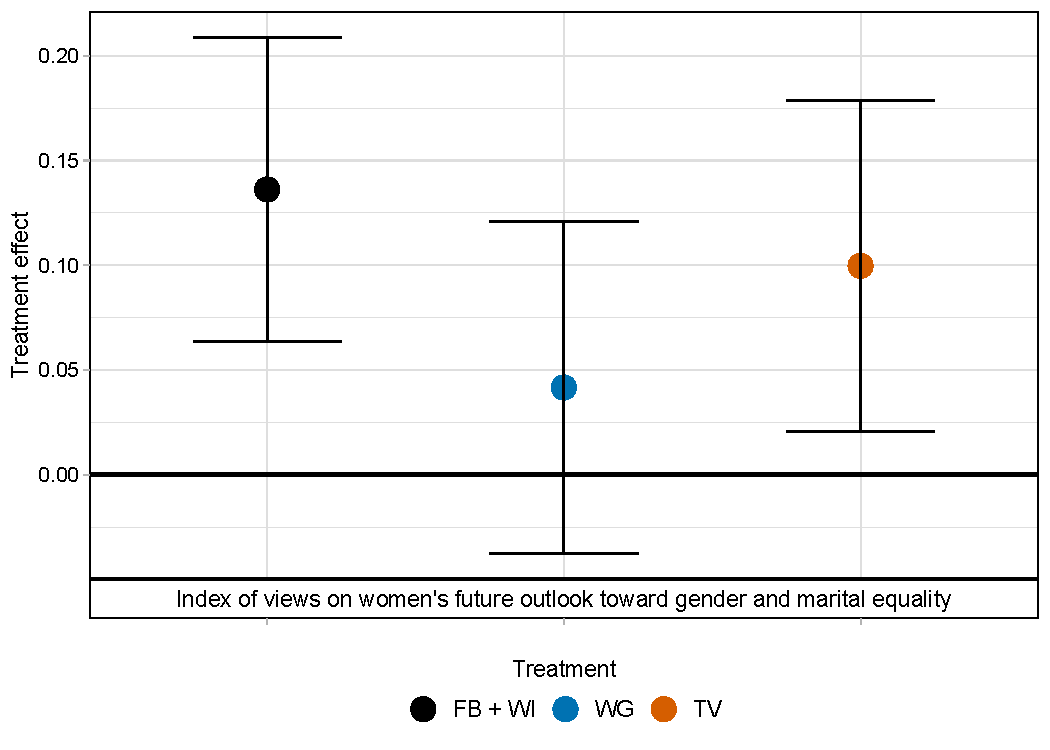
\includegraphics[width=12cm, height=9cm\textwidth]{Figures/RF-FS/Figure5.pdf}
        \captionsetup{width=.75\linewidth}
    \caption*{\footnotesize \textit{Notes:} The estimates and $95$\% confidence intervals in each box are from separate WGLS regressions where the weights are in the inverse probability of treatment assignment. The labels are the corresponding dependent variables regressed on treatment indicators (FB $+$ WI $=$ Facebook or WhatsApp individual message, WG $=$ WhatsApp group message, TV $=$ TV show reminder), relevant baseline controls and randomization block fixed effects. The outcomes included in the index of views on women's future outlook toward gender and marital equality are in Table S$23$.}
\end{figure}

\clearpage
 
\begin{figure}[H]
\caption{Comparison of attitudes and behavior between Arab Barometer and experimental sample respondents}
   \begin{minipage}{1\textwidth} 
   \begin{subfigure}[b]{0.48\linewidth}
    \centering
    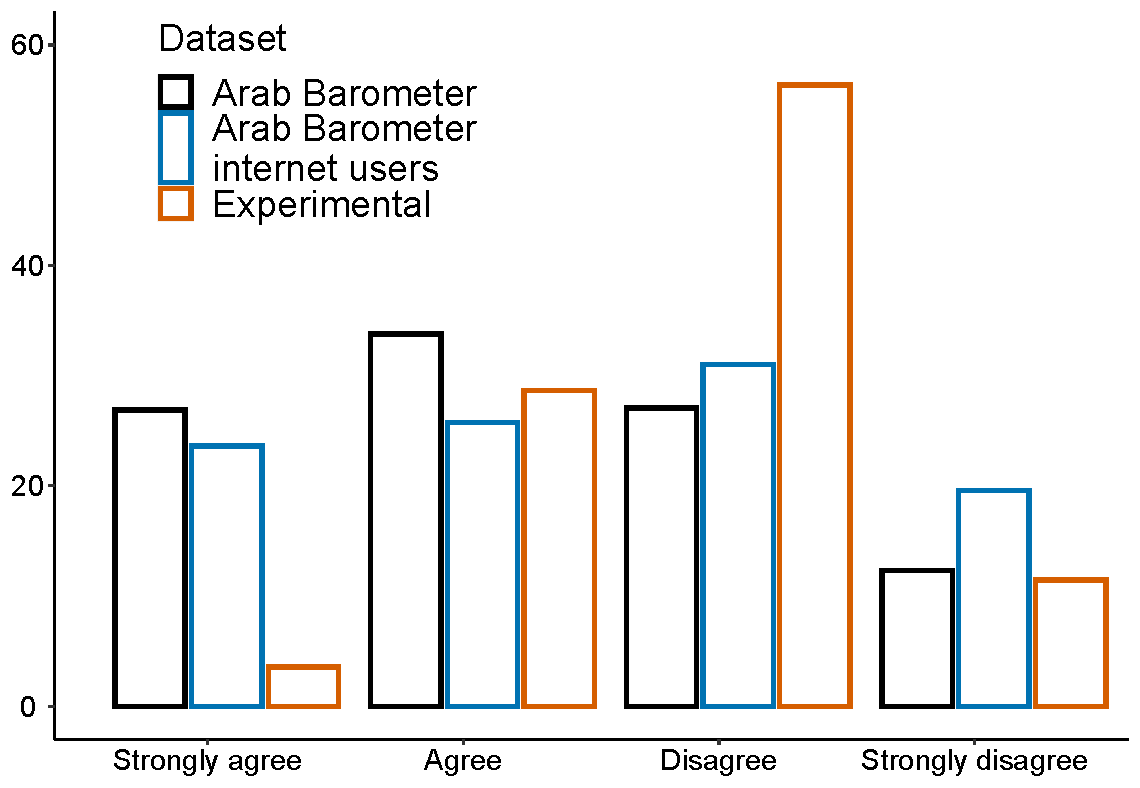
\includegraphics[height=6cm,width=8cm\linewidth]{Figures/AB/white/husb_fs.pdf} 
    \caption{Husband final say} 
    \label{} 
  \end{subfigure}
  \hspace{\fill}
  \begin{subfigure}[b]{0.48\linewidth}
    \centering
    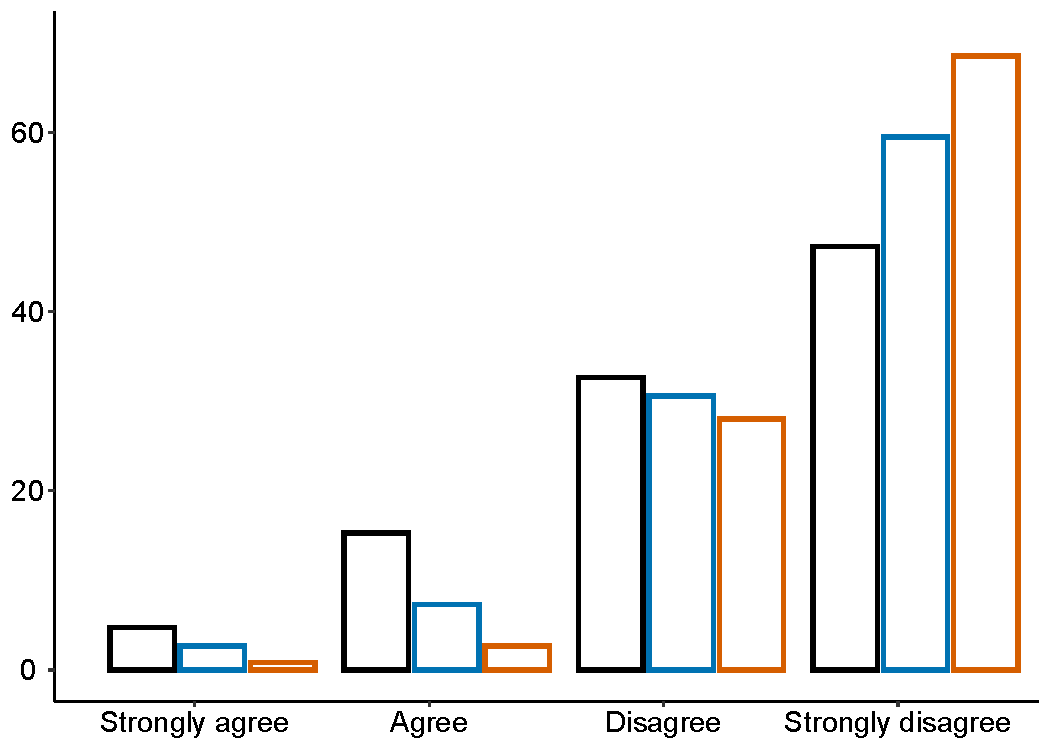
\includegraphics[height=6cm,width=8cm\linewidth]{Figures/AB/white/prio_educ.pdf} 
    \caption{Male education priority} 
    \label{} 
  \end{subfigure} 
   \begin{subfigure}[b]{0.48\linewidth}
    \centering
    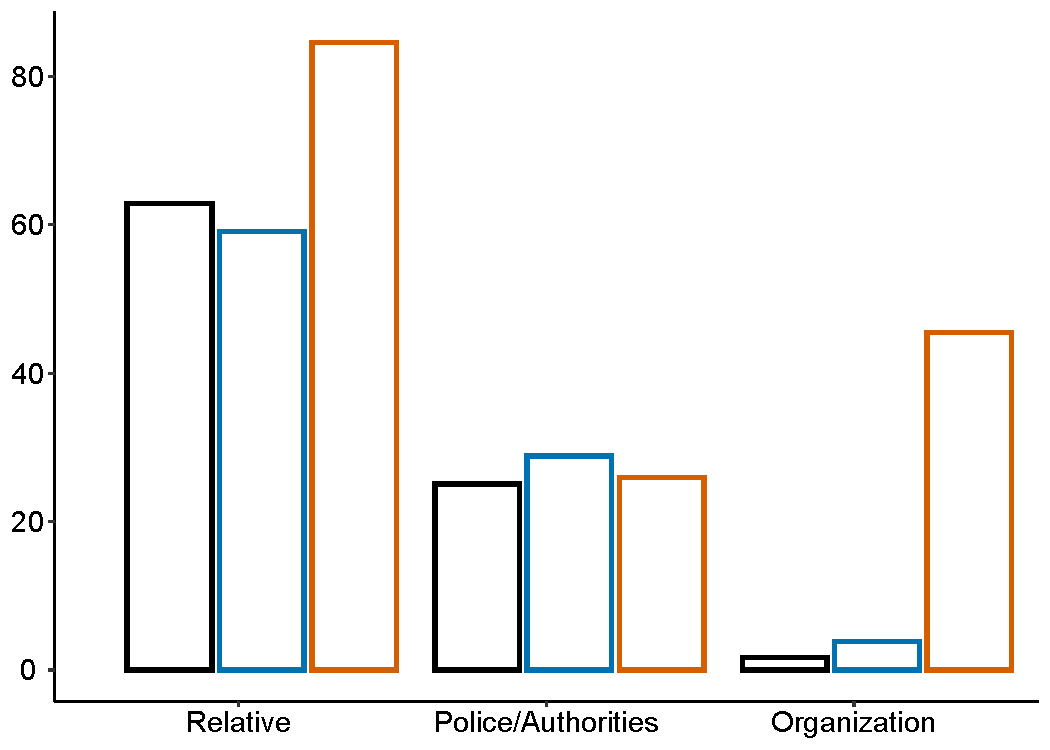
\includegraphics[height=6cm,width=8cm\linewidth]{Figures/AB/white/support.pdf} 
    \caption{Support from} 
    \label{} 
  \end{subfigure}
  \hspace{\fill}
  \begin{subfigure}[b]{0.48\linewidth}
    \centering    
    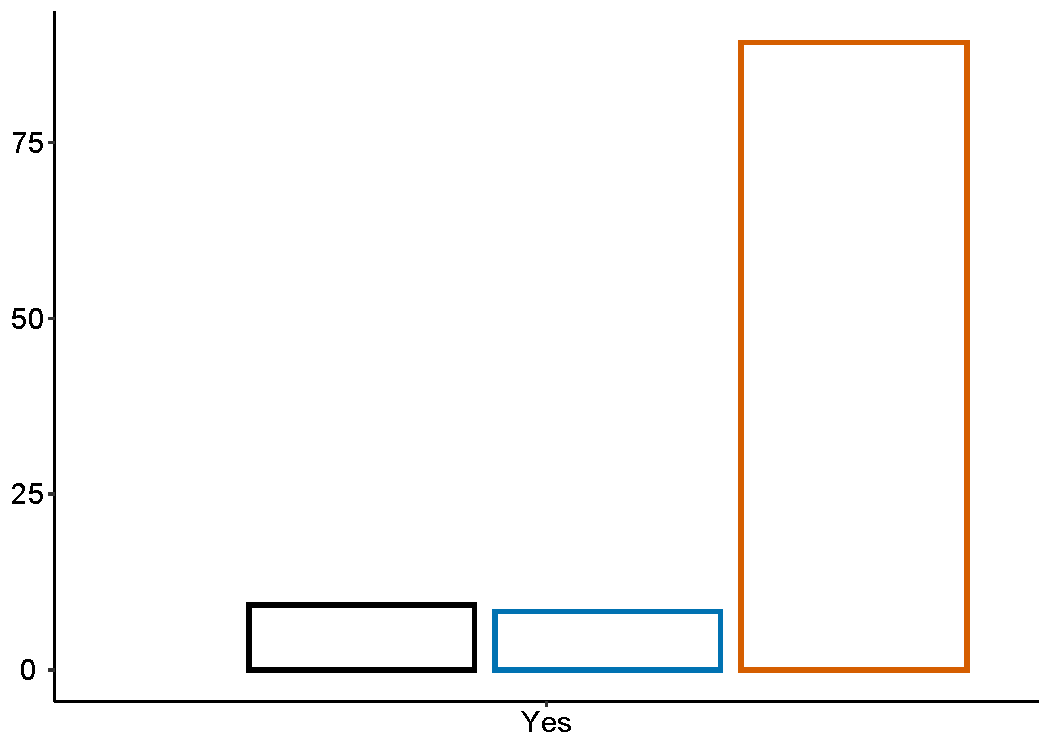
\includegraphics[height=6cm,width=8cm\linewidth]{Figures/AB/white/violence.pdf} 
    \caption{Experienced violence} 
    \label{} 
  \end{subfigure} 
\floatfoot{\footnotesize 
    \textit{Notes:} %\textsuperscript{1}
    The Arab Barometer data belongs to the $2016$ and $2018$ waves.  Additional summary statistic comparisons are in Table S$4$. 
    The “Support from” variables differ in both surveys: the Arab Barometer survey asked whether respondents thought that a family member who was abused would be able to receive assistance from each of the actors, and our survey asked whether respondents would recommend a friend or family member who was abused to reach each of the actors. $(2)$ The “Experienced violence” variable differs in both surveys: the Arab Barometer survey asked if in the last twelve months a female member of the household was abused by another member, and our survey asked whether, in the month before the COVID-19 pandemic, they heard of someone or themselves experienced being hit by a man.}
\end{minipage}
  \label{}
\end{figure}
 
  

\clearpage


\appendix


\section*{Supplementary Materials}
\setcounter{figure}{0}
\renewcommand{\figurename}{Fig.}
\renewcommand{\thefigure}{S\arabic{figure}}


\begin{figure}[H]
\caption{Survey responses by Egyptian Governorate. \label{fig:map}}
\centerline{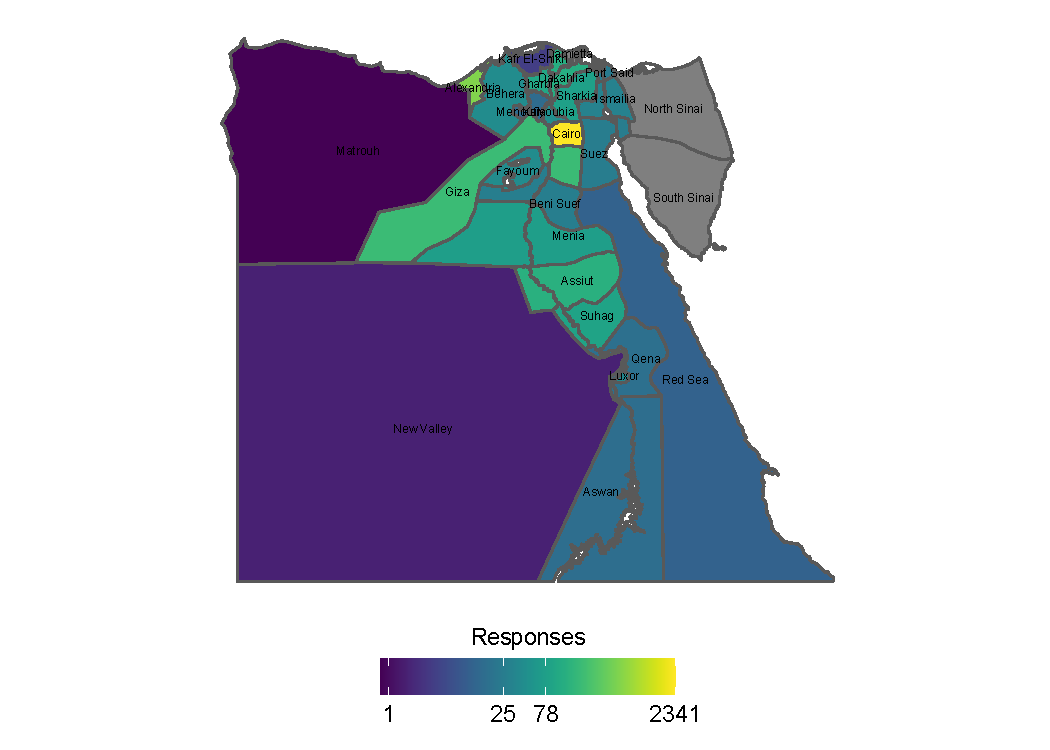
\includegraphics[width=1.15\textwidth]{Figures/Other/map_plot.pdf}}

\end{figure}


\begin{figure}[H]
\caption{Example of a treatment video whose link was disseminated to individuals assigned to the Facebook, WhatsApp Individual, and WhatsApp Group treatments.}
\centerline{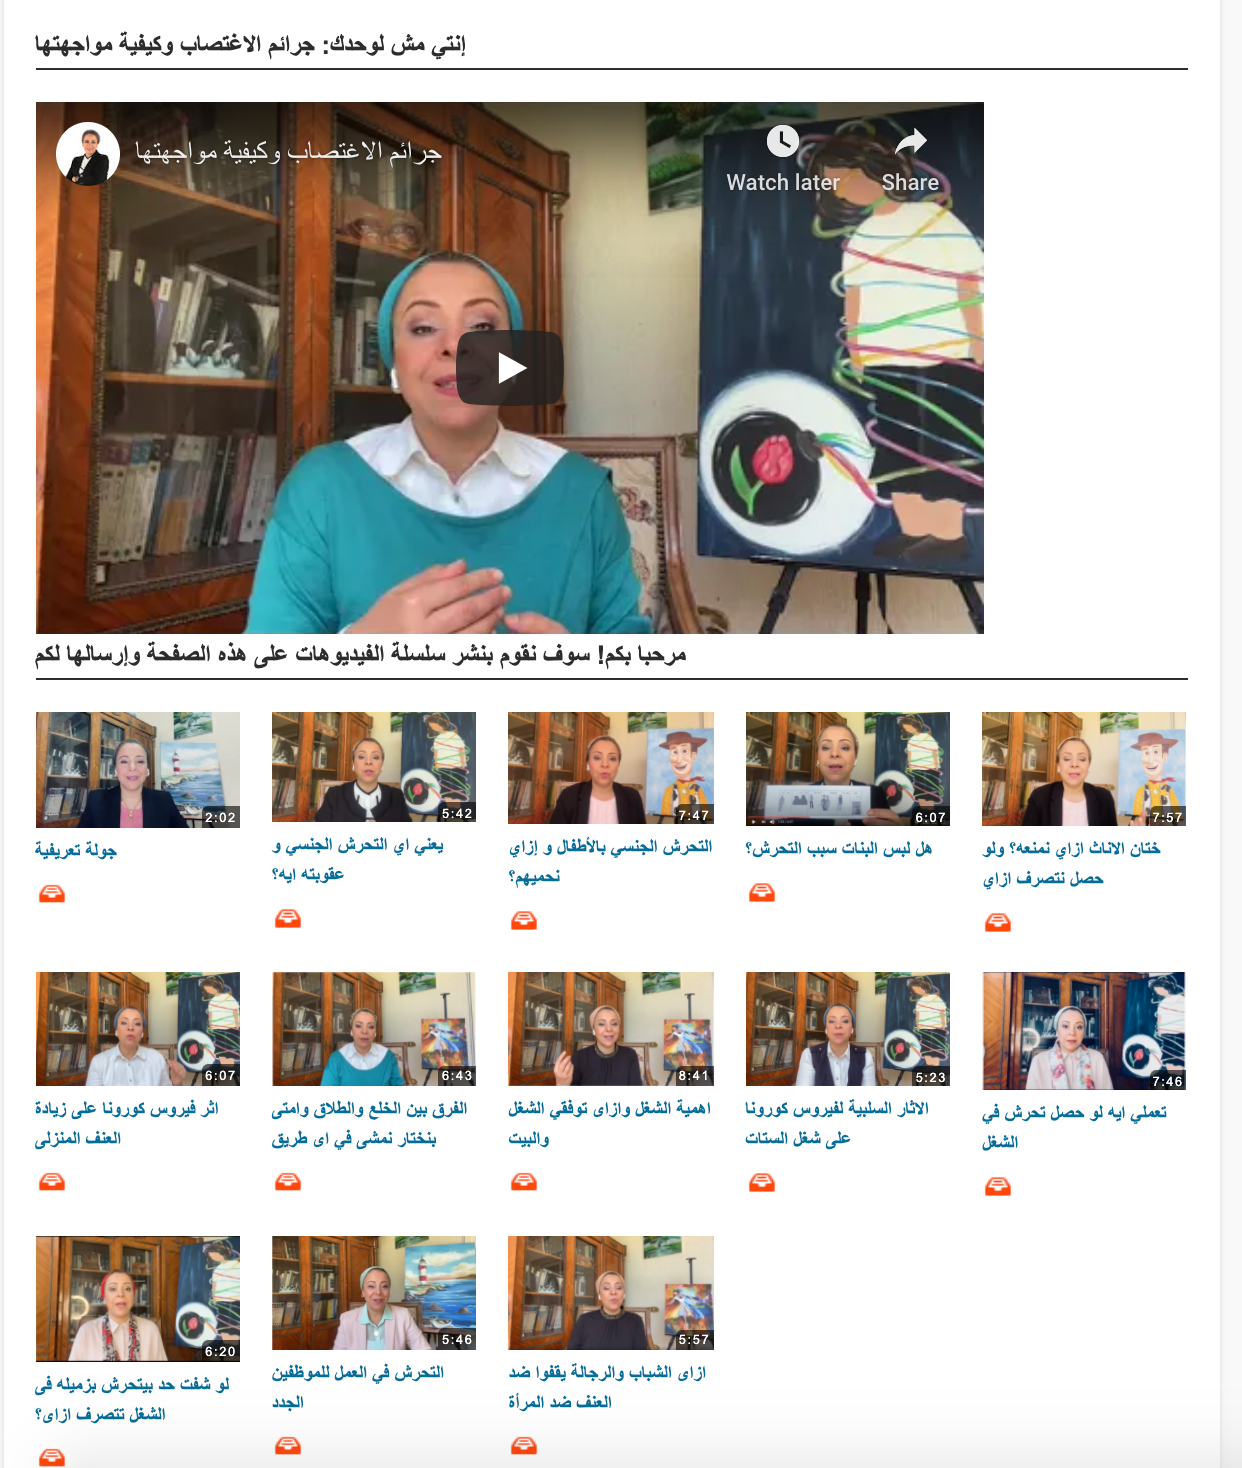
\includegraphics[width=0.7\textwidth,  keepaspectratio, clip=true, trim = 30 50 30 30]{Figures/Other/v6wg.png}}

\label{fig:mshlwa7dek.org}
\end{figure}



\begin{figure}[H]
\caption{Video landing web page visits for Facebook and WhatsApp Individual treatment before and after participants assigned to the Facebook treatment were shifted to the WhatsApp Individual treatment} 
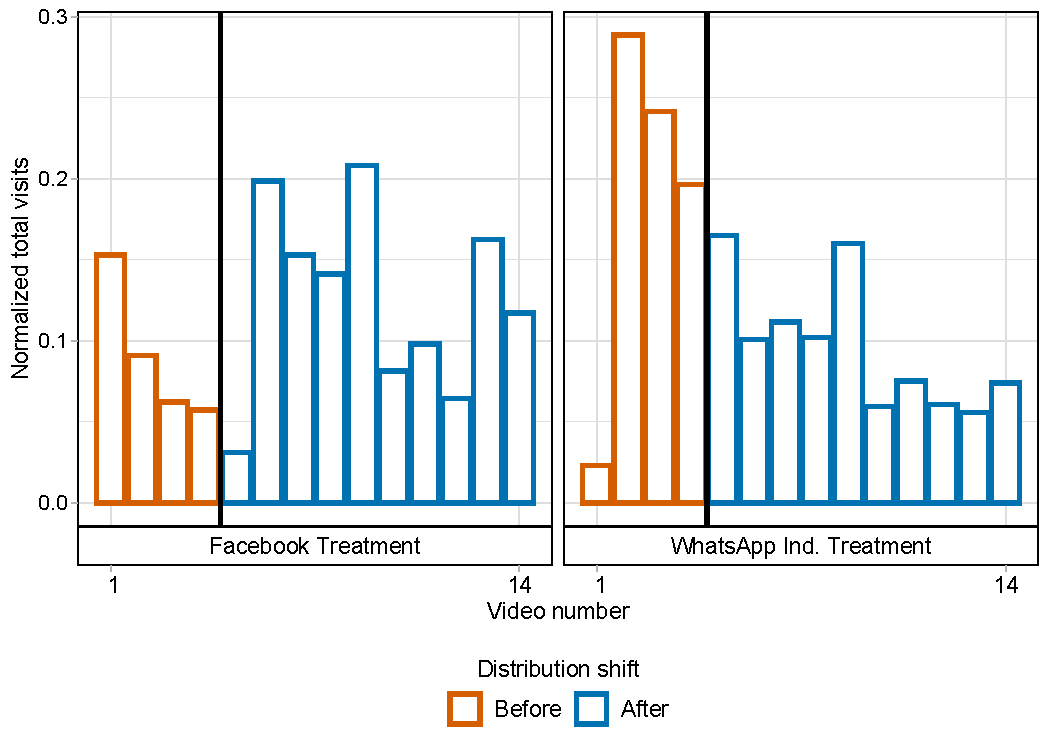
\includegraphics[width=1\textwidth]{Figures/Other/dist_change.pdf}
\captionsetup{width=.85\linewidth}
\label{fig:fb_shifts}
\end{figure}


\begin{figure}[H]
    \centering
    \caption{Difference in difference effects of WhatsApp Individual treatment on video landing web page visits}
    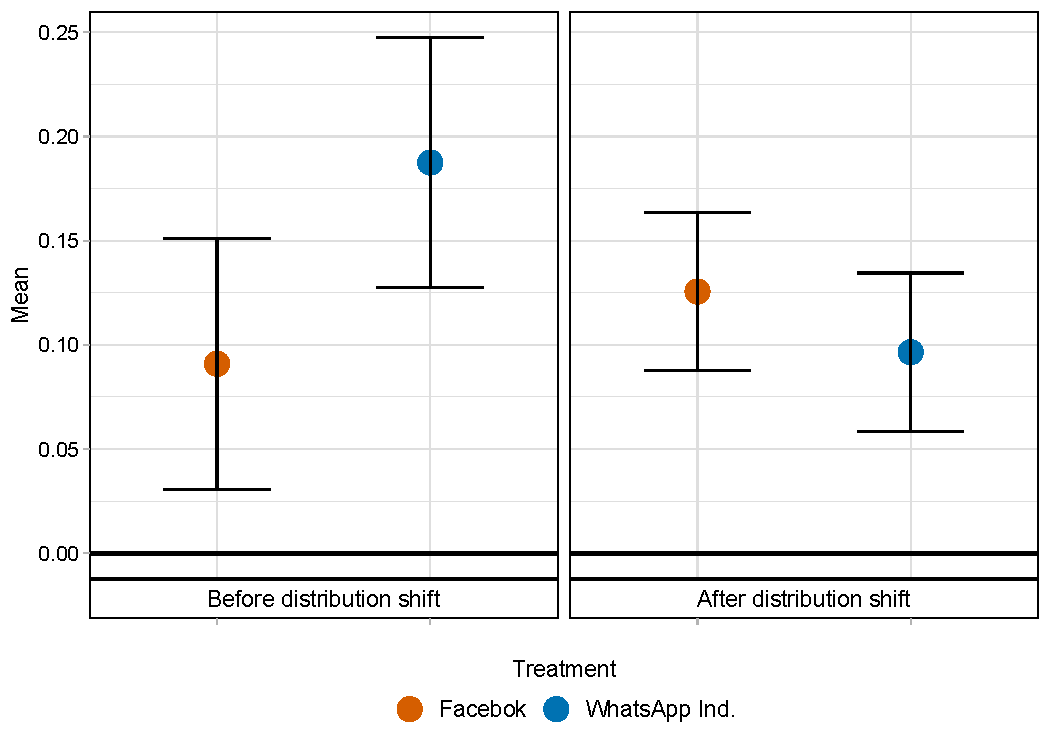
\includegraphics[width=12cm, height=9cm\textwidth]{Figures/Other/dist_dotted.pdf}
    \captionsetup{width=.75\linewidth}
    \caption*{\footnotesize  \textit{Notes:} The estimates and $95$\% confidence intervals in each box are from the same difference in difference regression. We regressed number of visits per assigned participant per video on an indicator for Facebook treatment assignment, an indicator for the shift in distribution from Facebook to WhatsApp Individual, and the interaction between the two indicators, while including video fixed effects. The coefficient on the interaction is $0.126$ (p $< 0.05$).}
\end{figure}



\begin{figure}[H]
\caption{Number of treatment web pages visited per web page user across treatments}   
   \begin{subfigure}[b]{0.48\linewidth}
    \centering
    \caption{All treatment pages} 
    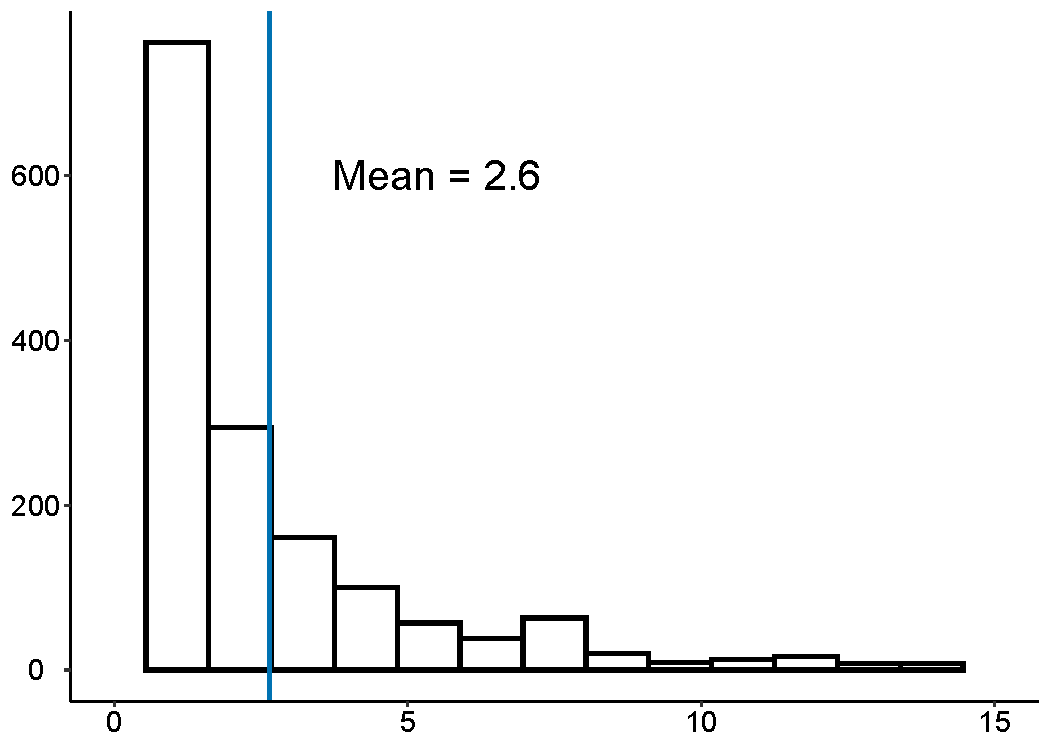
\includegraphics[height=6cm,width=8cm\linewidth]{Figures/Other/pages_all.pdf} 
    \label{} 
  \end{subfigure}
  \hspace{\fill}
  \begin{subfigure}[b]{0.48\linewidth}
    \centering
    \caption{Facebook treatment pages} 
    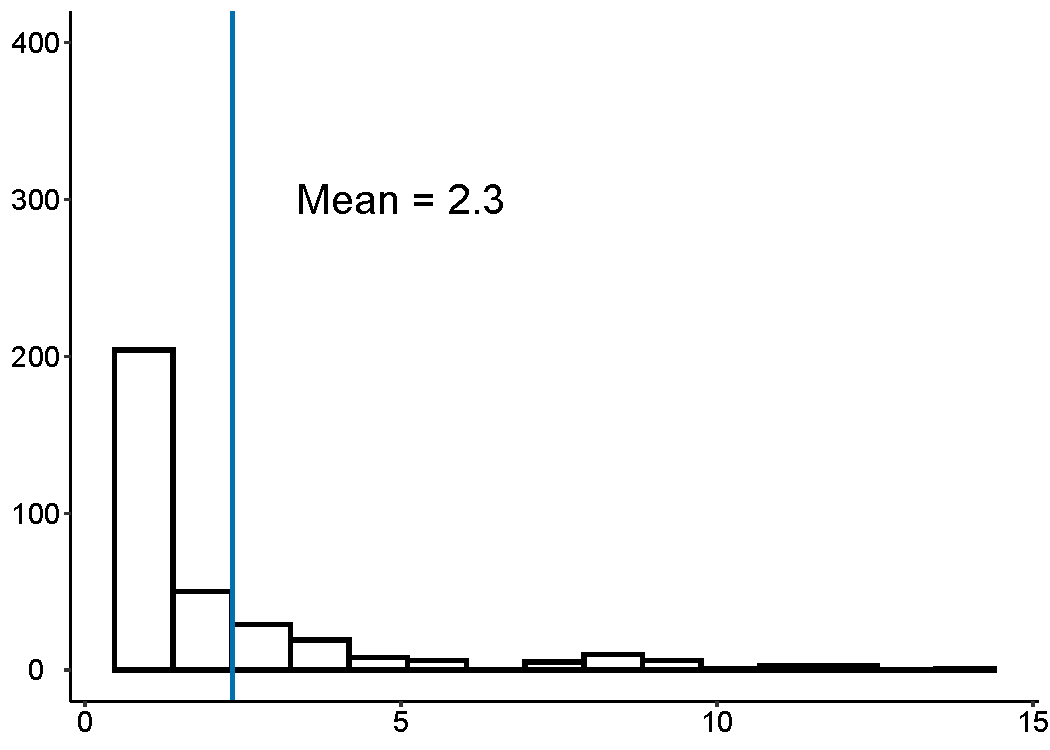
\includegraphics[height=6cm,width=8cm\linewidth]{Figures/Other/pages_fb.pdf} 
    \label{} 
  \end{subfigure} 
   \begin{subfigure}[b]{0.48\linewidth}
    \centering
    \caption{WhatsApp individual treatment pages} 
    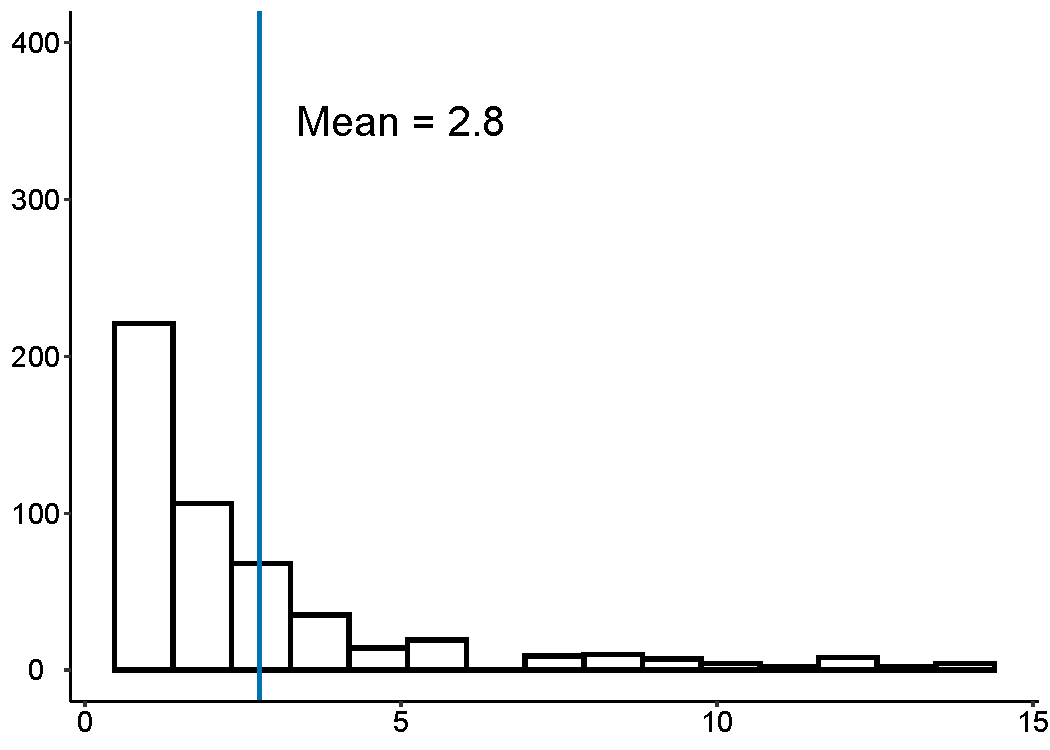
\includegraphics[height=6cm,width=8cm\linewidth]{Figures/Other/pages_wi.pdf} 
    \label{} 
  \end{subfigure}
  \hspace{\fill}
  \begin{subfigure}[b]{0.48\linewidth}
    \centering    
    \caption{WhatsApp group treatment pages} 
    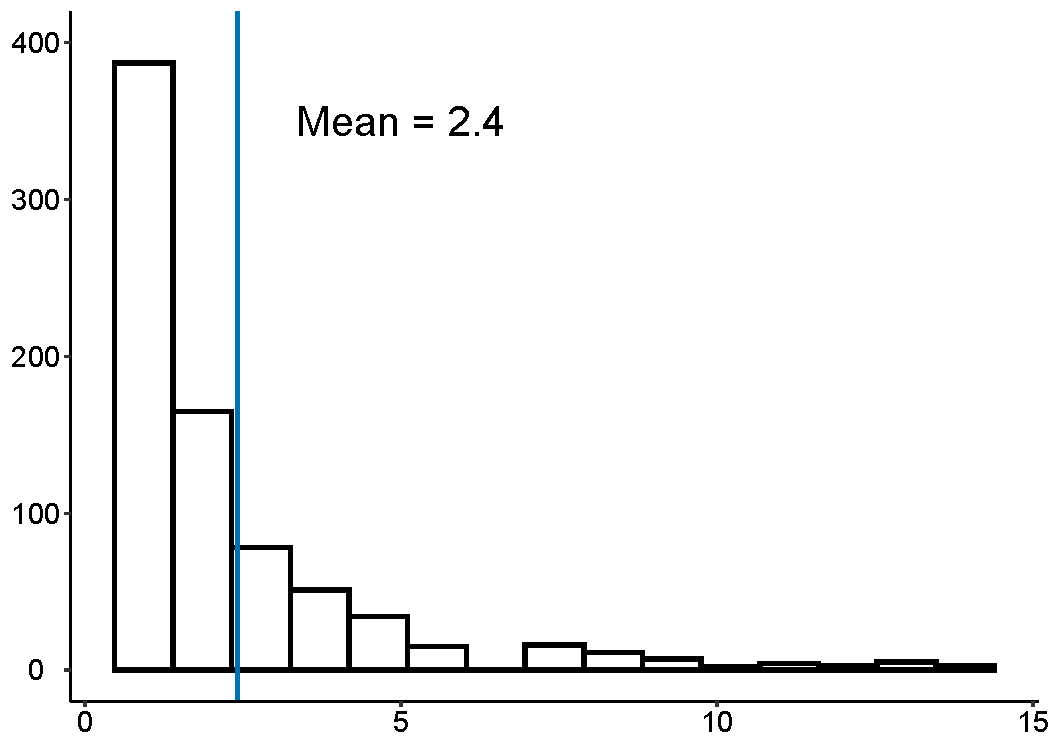
\includegraphics[height=6cm,width=8cm\linewidth]{Figures/Other/pages_wg.pdf} 
    \label{figure:video_visits}
  \end{subfigure} 
  \label{}
\end{figure}





\begin{figure}[H]
    \centering
    \caption{Treatment effects on hypothetical talking to husband and family members, or reporting to authorities when responding to domestic and sexual violence}
    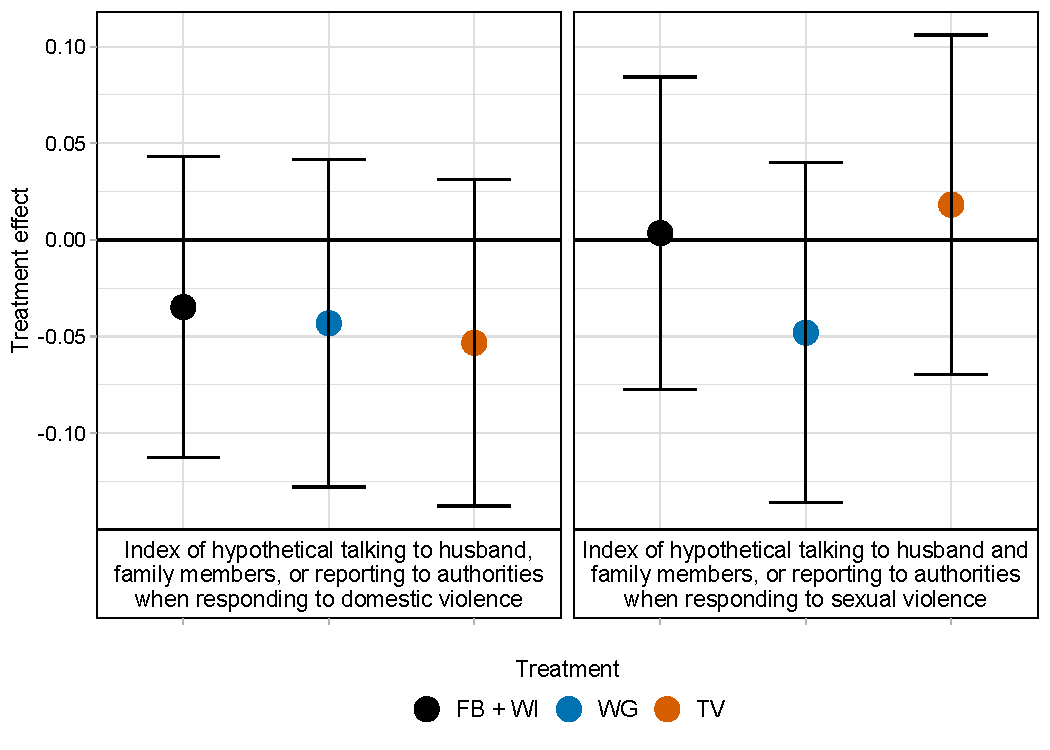
\includegraphics[width=12cm, height=9cm\textwidth]{Figures/RF-FS/FigureA1.pdf}
    \captionsetup{width=.75\linewidth}
    \caption*{\footnotesize  \textit{Notes:} The estimates and $95$\% confidence intervals in each box are from separate WGLS regressions where the weights are in the inverse probability of treatment assignment. The labels are the corresponding dependent variables regressed on treatment indicators (FB $+$ WI $=$ Facebook or WhatsApp individual message, WG $=$ WhatsApp group message, TV $=$ TV show reminder), relevant baseline controls and randomization block fixed effects. The outcomes included in the index of hypothetical talking to husband, family members, or reporting to authorities when responding to domestic violence are in Table S$24$. The outcomes included in the index of hypothetical talking to husband and family members, or reporting to authorities when responding to sexual violence are in Table S$25$.}
    
\end{figure}


\begin{figure}[H]
    \centering
    \caption{Treatment effects on violence experienced before COVID-19 and recent use of online resources or contact with an organization when responding to domestic or sexual violence}
    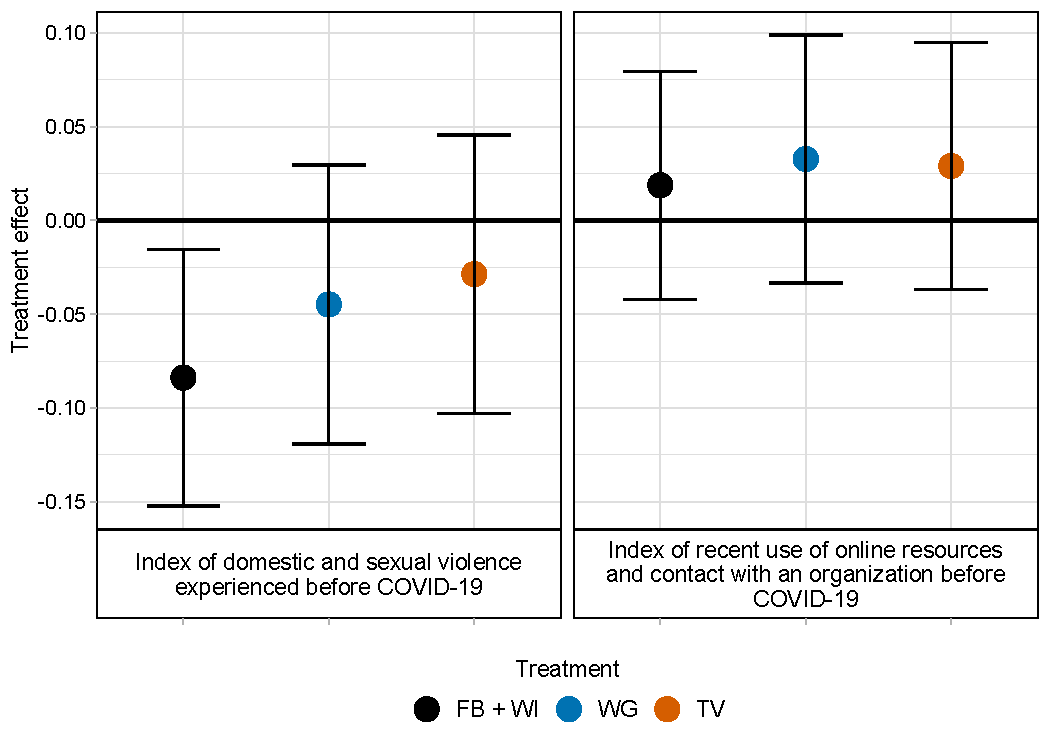
\includegraphics[width=12cm, height=9cm\textwidth]{Figures/RF-FS/FigureA2.pdf}
        \captionsetup{width=.75\linewidth}
    \caption*{\footnotesize \textit{Notes:} The estimates and 95\% confidence intervals in each box are from separate WGLS regressions where the weights are in the inverse probability of treatment assignment. The labels are the corresponding dependent variables regressed on treatment indicators (FB $+$ WI $=$ Facebook or WhatsApp individual message, WG $=$ WhatsApp group message, TV $=$ TV show reminder), relevant baseline controls and randomization block fixed effects. The outcomes included in the index of domestic and sexual violence experienced before COVID-19 are in Table S$26$. The outcomes included in the index of recent use of online resources and contact with an organization before COVID-19 are in Table S27.}
\end{figure}




\subsection*{Tables}
\setcounter{table}{0}
\renewcommand{\thetable}{S\arabic{table}}

\begin{table}[H]
\centering
\caption{Block sizes, treatment probabilities and responses rates by treatment assignment}
\label{table:randomization_proc}
\resizebox{\textwidth}{!}{
\begin{tabular}{lccccccc}
\hline
 &  & \multicolumn{2}{c}{\begin{tabular}[c]{@{}c@{}}With Facebook\\ account\end{tabular}} & \multicolumn{2}{c}{\begin{tabular}[c]{@{}c@{}}Only with WhatsApp\\ account\end{tabular}} &  &  \\ 
 \cmidrule(l{2pt}r{2pt}){3-4} \cmidrule(l{2pt}r{2pt}){5-6}
Treatment & Baseline & Block size & \begin{tabular}[c]{@{}l@{}}Treatment\\ probability\end{tabular} & Block size & \begin{tabular}[c]{@{}l@{}}Treatment\\ probability\end{tabular} &  Endline & Response Rate \\ 
Control & 1104 & 10 & 1/5 & 50 & 1/5 & 839 & 0.76 \\ 
Facebook & 565 & 10 & 3/5 & 0 & 0 & 418 & 0.74 \\ \begin{tabular}[c]{@{}l@{}}WhatsApp\\ Individual\end{tabular} & 1118 & 10 & 1/5 & 50 & 1/5 &   824 & 0.737 \\ 
\begin{tabular}[c]{@{}l@{}}WhatsApp\\ Group\end{tabular} & 1879 & 0 & 0 & 50 & 2/5 & 1382 & 0.735 \\ 
\begin{tabular}[c]{@{}l@{}}TV Show \\ Reminder\end{tabular} & 952 & 0 & 0 & 50 & 1/5  & 702 & 0.737 \\ \hline 
Total & 5618 &  &  &  &   & 4165 & 0.741 \\ \hline
\end{tabular}}\captionsetup{width=0.95\linewidth}
\caption*{\footnotesize \textit{Notes:} We block randomized treatment assignment separately according to whether we could identify the Facebook account of the baseline survey respondent.}
\end{table}


\begin{table}[H]
\centering
\caption{Unique Ips, users, visits, and average visit time by treatment assignment}
\resizebox{\textwidth}{!}{

\begin{tabular}{lccccc}
\hline
Treatmentassignment & Assigned &  Unique IPs & Unique users & Total visits & Average visit time \\ \hline
Facebook & 586 & 597 & 345 & 1347 & 4:02 \\
WhatsApp Individual & 1163 & 1178 & 509 & 2463 & 4:01 \\
WhatsApp Group& 1946 & 1671 & 781 & 3280 & 3:57 \\ \hline \hline
Total & 3695 & 3446 & 1635 & 7090 & 4:01 \\ \hline
\end{tabular} }
\captionsetup{width=0.95\linewidth}
\caption*{\footnotesize \textit{Notes:} Website data provides the number of unique IPs, unique users, and total visits by treatment assignment. A Unique User is determined via cookies and thus corresponds to a specific individual in a particular device. Note that this table reports different treatment assignment numbers than Table S$1$ as it includes assignments to individuals who responded twice to the endline survey, and thus were excluded from the study.}
\label{table:website_visits}
\end{table}



\begin{table}[H]
\centering
\caption{Website and YouTube analytics}
\resizebox{\textwidth}{!}{
    \begin{tabular}{p{6cm}p{1.5cm}p{1.5cm}p{1.5cm}{1.5cm}}
\hline
 \multicolumn{1}{l}{} & \multicolumn{2}{c}{Website} & \multicolumn{2}{c}{YouTube} \\
 \cmidrule(l{2pt}r{2pt}){2-3} \cmidrule(l{2pt}r{2pt}){4-5}
Video & \multicolumn{1}{l}{Visits} & \multicolumn{1}{l}{\begin{tabular}[c]{@{}l@{}}Average visit\\ time\end{tabular}} & \multicolumn{1}{l}{Views} & \multicolumn{1}{l}{\begin{tabular}[c]{@{}l@{}}Average viewing\\ time\end{tabular}} \\ \hline
What is sexual harassment and what is its penalty? &  682 & 0:03:33 & 535 & 0:02:33 \\
Sexual harassment of children and how to protect them? &  493 & 0:04:57 & 391 & 0:03:44 \\
Are women's clothes the cause of sexual harassment? &  372 & 0:03:29 & 324 & 0:02:49 \\
Female genital cutting and how to stop it? &  286 & 0:04:39 & 268 & 0:04:04 \\
Impact of COVID-19 on increasing domestic violence & 265 & 0:04:33 & 212 & 0:02:47 \\
Rape crimes and how to fight them and COVID-19 & 226 & 0:03:11 & 207 & 0:02:53 \\
The difference between divorce and Khul and when to choose either? &  230 & 0:04:50 & 268 & 0:03:22 \\
The importance of work and how to balance work and family life? & 268 & 0:04:47 & 281 & 0:03:51 \\
The negative effects of Covid-19 on women’s work & 96 & 0:02:52 & 107 & 0:02:55 \\
How to deal with workplace harassment? &  143 & 0:04:33 & 175 & 0:03:22 \\
How to act if you saw someone harassing a colleague at work? & 110 & 0:4:17 & 146 & 0:02:55 \\
Dealing with workplace harassment for new employees & 146 & 0:04:20 & 172 & 0:02:44 \\
How can men stand against violence against women? & 184 & 0:06:51 & 184 & 0:02:33 \\ \hline \hline
Total  \multicolumn{1}{l}{} & 3471 & 0:04:22 & 3270 & 0:02:59 \\ \hline
\end{tabular}}
\captionsetup{width=0.95\linewidth}
\caption*{\footnotesize \textit{Notes:} Website and YouTube analytics show that videos received a higher number of website visits and viewing time than YouTube views. The reason is that and the website measures total duration on the site, whereas YouTube measures time spent viewing the content and is much stricter in defining whether a video was viewed.}

\end{table}





\begin{table}[H]
\centering
\vspace*{-1.5cm} \caption{Summary statistics of comparable demographics both in the Arab Barometer sample, the Arab Barometer internet user sample, and the experimental sample.}
\scriptsize
\scalebox{1.25}{
\begin{tabular}{lcccc}
\hline
 & \begin{tabular}[c]{@{}l@{}}Arab Barometer \\ sample\end{tabular}   & 
 \begin{tabular}[c]{@{}l@{}}Arab Barometer \\internet user sample\end{tabular} & 
 \begin{tabular}[c]{@{}l@{}}Experimental  \\ sample\end{tabular} & 
 \begin{tabular}[c]{@{}l@{}}Arab Barometer  \\ survey years\end{tabular}   \\ \hline
Age & 38.457    & 30.238    & 31.598  & 2016, 2018 \\
& 13.930   & 10.440 & 9.137 &   \\
& 1,826 & 792  & 4,165  &    \\ \hline
Education  & 3.352  & 4.701    & 5.344  & 2016, 2018 \\
& 1.768  & 1.225  & 1.179   &     \\
& 1,861  & 801  & 4,165    &  \\ \hline
Whether single  & 0.176 & 0.341  & 0.290   & 2016, 2018 \\
 & 0.381  & 0.475  &  0.454  &   \\
& 1,861  & 801    & 4,165   &      \\ \hline
Whether engaged  & 0.053 &  0.114 & 0.044   & 2016, 2018 \\
 & 0.225  & 0.318  & 0.205   &   \\
& 1,861  & 801    & 4,165   &      \\ \hline
Whether married  & 0.606 & 0.479  &  0.570  & 2016, 2018 \\
 & 0.489  & 0.500  &  0.495  &   \\
& 1,861  & 801    & 4,165   &      \\ \hline
Whether separated  & 0.047 &  0.047 &  0.081  & 2016, 2018 \\
 & 0.211  &  0.213 &  0.272  &   \\
& 1,861  & 801    & 4,165   &      \\ \hline
Whether widowed  & 0.118 &  0.019 &  0.016  & 2016, 2018 \\
 &  0.322 & 0.137  & 0.124   &   \\
& 1,861  & 801    & 4,165   &      \\ \hline
Social status  & 3.911  & 2.992  & 3.253   & 2016, 2018 \\
 & 3.049   & 1.565  & 1.556   &   \\
& 1,861  & 801    & 4,165  &     \\ \hline
Number of children   & 1.090     & 0.916 & 1.274    & 2016, 2018 \\
& 1.376     & 1.235  & 1.327   &    \\
& 1,861  & 801    & 4,165   &      \\ \hline
Facebook  & 0.372   & 0.877 & 0.884    & 2016, 2018 \\
& 0.484   & 0.328   & 0.321  &   \\
& 1,861  & 801   & 4,165  &    \\ \hline
WhatsApp   & 0.303   & 0.648   & 0.857   & 2018       \\
& 0.460  & 0.478   & 0.351      &     \\
& 1,200      & 598    & 4,165       &            \\ \hline
YouTube   & 0.220     & 0.471  & 0.387    & 2018   \\
& 0.415     & 0.500  & 0.487      &            \\
& 1,200      & 598  & 4,165       &            \\ \hline
Instagram     & 0.117     & 0.276    & 0.199      & 2016, 2018 \\
 & 0.321     & 0.447  & 0.399      &        \\
& 1,861      & 801    & 4,165   &        \\ \hline
Twitter  & 0.111     & 0.262  & 0.080   & 2016, 2018 \\
 & 0.315     & 0.440    & 0.272    &       \\
 & 1,861      & 801   & 4,165   &      \\ \hline
Snapchat& 0.040     & 0.085  & 0.043   & 2018    \\
& 0.195     & 0.279  & 0.203     &       \\
& 1,200      & 598    & 4,165   &     \\ \hline
Hours spent on social media   & 1.747   & 2.595                                                           & 2.879      & 2018       \\
& 0.942     & 0.737 & 0.896   &   \\
& 1,200    & 598   & 4,165    &  \\ \hline 
\end{tabular}}
\captionsetup{width=1\linewidth}
\caption*{\footnotesize \textit{Notes:} For every variable, each row shows the mean, standard deviation, and number of observations.}
\end{table}






% Balance Tables --------------------------------------------------

\subsubsection*{Balance Tables}

\begin{table}[H] \centering 
  \caption{Balance on demographics variables} 
  \label{} 
\footnotesize 
\begin{tabular}{@{\extracolsep{2pt}}lD{.}{.}{-3} D{.}{.}{-3} D{.}{.}{-3} D{.}{.}{-3} D{.}{.}{-3} } 
\\[-1.8ex]\hline 
\hline \\[-1.8ex] 
\\[-0.5ex] 
\multicolumn{6}{l}{\textbf{Panel A: Respondent’s outcomes}} \\
\hline \\[-1ex]  
 & \multicolumn{1}{c}{Age} & \multicolumn{1}{c}{\shortstack{Education \\ (BA)}} & \multicolumn{1}{c}{\shortstack{Number \\ of male \\ children}} & \multicolumn{1}{c}{\shortstack{Number \\ of female \\ children}} & \multicolumn{1}{c}{\shortstack{Other \\ family \\members}} \\ 
\\[-1.8ex] & \multicolumn{1}{c}{(1)} & \multicolumn{1}{c}{(2)} & \multicolumn{1}{c}{(3)} & \multicolumn{1}{c}{(4)} & \multicolumn{1}{c}{(5)}\\ 
\hline \\[-1.8ex] 
 Facebook and \\ WhatsApp Ind. & 0.096 & -0.021 & -0.028 & 0.062^{*} & -0.135 \\ 
  & (0.363) & (0.013) & (0.035) & (0.035) & (0.125) \\ 
  & & & & & \\ 
 WhatsApp Group & -0.008 & -0.012 & -0.014 & 0.021 & -0.050 \\ 
  & (0.396) & (0.014) & (0.038) & (0.038) & (0.136) \\ 
  & & & & & \\ 
 TV Show Reminder & -0.144 & -0.020 & -0.058 & 0.027 & -0.141 \\ 
  & (0.395) & (0.014) & (0.038) & (0.037) & (0.136) \\ 
  & & & & & \\ 
\hline \\[-1.8ex] 
Control Mean & 31.507 & 0.753 & 0.685 & 0.559 & 2.652 \\ 
Observations & \multicolumn{1}{c}{4,165} & \multicolumn{1}{c}{4,165} & \multicolumn{1}{c}{4,165} & \multicolumn{1}{c}{4,165} & \multicolumn{1}{c}{4,165} \\ 
R$^{2}$ & \multicolumn{1}{c}{0.161} & \multicolumn{1}{c}{0.518} & \multicolumn{1}{c}{0.136} & \multicolumn{1}{c}{0.120} & \multicolumn{1}{c}{0.101} \\ 
\hline 
\\[-0.5ex] 
\multicolumn{6}{l}{\textbf{Panel B: Whether married and husband’ outcomes}} \\
\hline \\[-1ex]  
 & \multicolumn{1}{c}{Married} & \multicolumn{1}{c}{Age} & \multicolumn{1}{c}{\shortstack{Education \\(BA)}} & \multicolumn{1}{c}{\shortstack{Marriage \\ duration}} & \multicolumn{1}{c}{\shortstack{Husband \\ lives \\ at home}} \\ 
\\[-1.8ex] & \multicolumn{1}{c}{(1)} & \multicolumn{1}{c}{(2)} & \multicolumn{1}{c}{(3)} & \multicolumn{1}{c}{(4)} & \multicolumn{1}{c}{(5)}\\ 
\hline \\[-1.8ex] 
 Facebook and \\ WhatsApp Ind. & 0.012 & 7.235^{*} & -0.035^{**} & -0.336 & 0.021 \\ 
  & (0.017) & (4.352) & (0.017) & (0.431) & (0.023) \\ 
  & & & & & \\ 
 WhatsApp Group & 0.005 & 2.469 & -0.053^{***} & -0.091 & 0.032 \\ 
  & (0.018) & (4.614) & (0.018) & (0.456) & (0.024) \\ 
  & & & & & \\ 
 TV Show Reminder & 0.002 & -1.299 & -0.042^{**} & 0.427 & 0.018 \\ 
  & (0.018) & (4.660) & (0.018) & (0.461) & (0.024) \\ 
  & & & & & \\ 
\hline \\[-1.8ex] 
Control Mean & 0.555 & 31.631 & 10.064 & 0.798 & 0.818 \\ 
Observations & \multicolumn{1}{c}{4,165} & \multicolumn{1}{c}{2,348} & \multicolumn{1}{c}{2,354} & \multicolumn{1}{c}{2,354} & \multicolumn{1}{c}{2,354} \\ 
R$^{2}$ & \multicolumn{1}{c}{0.401} & \multicolumn{1}{c}{0.057} & \multicolumn{1}{c}{0.561} & \multicolumn{1}{c}{0.163} & \multicolumn{1}{c}{0.079} \\ 
\hline 
\hline \\[-1.8ex] 
\multicolumn{6}{l} {\parbox[t]{11cm}{ \textit{Notes:} 
We report estimates from WGLS regressions where the weights are in the inverse probability of treatment assignment, including randomization block fixed effects. * denotes p$<$0.1, ** denotes p$<$0.05, and *** denotes p$<$0.01.}} \\
\end{tabular} 
\end{table} 




\begin{table}[H] \centering 
  \caption{Balance on before and during COVID-19 home presence of respondent and husband, and whether household income declined with COVID-19} 
  \label{} 
\footnotesize 
\hspace*{-1cm}\begin{tabular}{@{\extracolsep{2pt}}lD{.}{.}{-3} D{.}{.}{-3} D{.}{.}{-3} D{.}{.}{-3} D{.}{.}{-3} D{.}{.}{-3} D{.}{.}{-3} D{.}{.}{-3} D{.}{.}{-3} } 
\\[-1.8ex]\hline 
\hline \\[-1.8ex] 
 & \multicolumn{9}{c}{\textit{Dependent variable:}} \\ 
\cline{2-10} 
 & \multicolumn{4}{c}{Before COVID-19} & \multicolumn{4}{c}{During COVID-19} \\
 \cmidrule{2-5}  \cmidrule{6-9} 
  & \multicolumn{1}{c}{\shortstack{full time\\ at home}} & 
  \multicolumn{1}{c}{\shortstack{partially\\ at home}} & 
  \multicolumn{1}{c}{\shortstack{husband \\full time \\at home}} & 
  \multicolumn{1}{c}{\shortstack{husband \\ partially\\ at home}} & 
  \multicolumn{1}{c}{\shortstack{full time \\at home}} & 
  \multicolumn{1}{c}{\shortstack{partially\\ at home}} & 
  \multicolumn{1}{c}{\shortstack{husband  \\full time \\at home}} & 
  \multicolumn{1}{c}{\shortstack{husband  \\partially\\ at home}} & 
  \multicolumn{1}{c}{\shortstack{COVID-19 \\income \\decline}} \\ 
\\[-1.8ex] & \multicolumn{1}{c}{(1)} & \multicolumn{1}{c}{(2)} & \multicolumn{1}{c}{(3)} & \multicolumn{1}{c}{(4)} & \multicolumn{1}{c}{(5)} & \multicolumn{1}{c}{(6)} & \multicolumn{1}{c}{(7)} & \multicolumn{1}{c}{(8)} & \multicolumn{1}{c}{(9)}\\ 
\hline \\[-1.8ex] 
 Facebook and \\ WhatsApp Ind. & -0.001 & 0.001 & 0.002 & 0.011 & -0.014 & 0.005 & 0.012 & 0.029 & 0.018 \\ 
  & (0.020) & (0.021) & (0.018) & (0.024) & (0.018) & (0.017) & (0.025) & (0.027) & (0.018) \\ 
  & & & & & & & & & \\ 
 WhatsApp Group & -0.017 & -0.003 & 0.017 & 0.002 & -0.013 & -0.001 & 0.054^{**} & -0.026 & 0.015 \\ 
  & (0.021) & (0.022) & (0.019) & (0.025) & (0.020) & (0.018) & (0.027) & (0.029) & (0.019) \\ 
  & & & & & & & & & \\ 
 TV Show Reminder & -0.035^{*} & 0.007 & 0.007 & -0.040 & -0.027 & 0.015 & 0.045^{*} & -0.062^{**} & 0.032^{*} \\ 
  & (0.021) & (0.022) & (0.019) & (0.025) & (0.020) & (0.018) & (0.027) & (0.029) & (0.019) \\ 
  & & & & & & & & & \\ 
\hline \\[-1.8ex] 
Control Mean & 0.366 & 0.45 & 0.099 & 0.221 & 0.745 & 0.194 & 0.228 & 0.344 & 0.757 \\ 
Observations & \multicolumn{1}{c}{4,162} & \multicolumn{1}{c}{4,162} & \multicolumn{1}{c}{2,351} & \multicolumn{1}{c}{2,351} & \multicolumn{1}{c}{4,165} & \multicolumn{1}{c}{4,155} & \multicolumn{1}{c}{2,346} & \multicolumn{1}{c}{2,346} & \multicolumn{1}{c}{4,165} \\ 
R$^{2}$ & \multicolumn{1}{c}{0.113} & \multicolumn{1}{c}{0.092} & \multicolumn{1}{c}{0.074} & \multicolumn{1}{c}{0.092} & \multicolumn{1}{c}{0.083} & \multicolumn{1}{c}{0.075} & \multicolumn{1}{c}{0.080} & \multicolumn{1}{c}{0.085} & \multicolumn{1}{c}{0.067} \\ 
\hline 
\hline \\[-1.8ex] 
\multicolumn{10}{l} {\parbox[t]{18cm}{ \textit{Notes:} 
We report estimates from WGLS regressions where the weights are in the inverse probability of treatment assignment, including randomization block fixed effects. * denotes p$<$0.1, ** denotes p$<$0.05, and *** denotes p$<$0.01.}} \\
\end{tabular} 
\end{table} 


\begin{table}[H] \centering 
  \caption{Balance on TV show consumption variables} 
  \label{} 
\footnotesize 
\hspace*{-1cm}\begin{tabular}{@{\extracolsep{2pt}}lD{.}{.}{-3} D{.}{.}{-3} D{.}{.}{-3} D{.}{.}{-3} D{.}{.}{-3} D{.}{.}{-3} D{.}{.}{-3} } 
\\[-1.8ex]\hline 
\hline \\[-1.8ex] 
 & \multicolumn{7}{c}{\textit{Dependent variable:}} \\ 
\cline{2-8} 
 & \multicolumn{1}{c}{\shortstack{Watches TV \\morning}} & \multicolumn{1}{c}{\shortstack{Watches TV \\afternoon}} & \multicolumn{1}{c}{\shortstack{Watches TV \\evening}} & \multicolumn{1}{c}{\shortstack{Own TV \\satellite}} & \multicolumn{1}{c}{\shortstack{Watches Channels \\ of TV show}} & \multicolumn{1}{c}{\shortstack{Watches TV\\show type}} & \multicolumn{1}{c}{\shortstack{Mentioned \\watched TV \\show Saturday \\evening}} \\ 
\\[-1.8ex] & \multicolumn{1}{c}{(1)} & \multicolumn{1}{c}{(2)} & \multicolumn{1}{c}{(3)} & \multicolumn{1}{c}{(4)} & \multicolumn{1}{c}{(5)} & \multicolumn{1}{c}{(6)} & \multicolumn{1}{c}{(7)}\\ 
\hline \\[-1.8ex] 
 All treatments & 0.010 & -0.029 & -0.011 & 0.009 & 0.014 & 0.039^{**} & 0.001 \\ 
  & (0.015) & (0.019) & (0.017) & (0.010) & (0.015) & (0.019) & (0.002) \\ 
  & & & & & & & \\ 
 in\_group\_10018 & 0.010 & -0.007 & -0.006 & 0.009 & 0.012 & 0.027 & 0.002 \\ 
  & (0.016) & (0.021) & (0.019) & (0.011) & (0.017) & (0.021) & (0.002) \\ 
  & & & & & & & \\ 
 reminder\_10018 & 0.013 & -0.045^{**} & -0.004 & -0.004 & -0.001 & 0.009 & 0.005^{**} \\ 
  & (0.016) & (0.021) & (0.019) & (0.011) & (0.017) & (0.021) & (0.002) \\ 
  & & & & & & & \\ 
\hline \\[-1.8ex] 
Control Mean & 0.137 & 0.319 & 0.781 & 0.934 & 0.148 & 0.267 & 0 \\ 
Observations & \multicolumn{1}{c}{4,165} & \multicolumn{1}{c}{4,165} & \multicolumn{1}{c}{4,165} & \multicolumn{1}{c}{4,165} & \multicolumn{1}{c}{4,165} & \multicolumn{1}{c}{4,165} & \multicolumn{1}{c}{4,165} \\ 
R$^{2}$ & \multicolumn{1}{c}{0.045} & \multicolumn{1}{c}{0.060} & \multicolumn{1}{c}{0.057} & \multicolumn{1}{c}{0.059} & \multicolumn{1}{c}{0.047} & \multicolumn{1}{c}{0.071} & \multicolumn{1}{c}{0.043} \\ 
\hline 
\hline \\[-1.8ex] 
\multicolumn{8}{l} {\parbox[t]{18cm}{ \textit{Notes:} 
We report estimates from WGLS regressions where the weights are in the inverse probability of treatment assignment, 
including randomization block fixed effects. * denotes p$<$0.1, ** denotes p$<$0.05, and *** denotes p$<$0.01.}} \\
\end{tabular} 
\end{table} 


\clearpage

\begin{table}[H] \centering 
  \caption{Balance on social media habits and videos received variables} 
  \label{} 
\footnotesize 
\hspace*{-2.65cm} \begin{tabular}{@{\extracolsep{0pt}}lD{.}{.}{-3} D{.}{.}{-3} D{.}{.}{-3} D{.}{.}{-3} D{.}{.}{-3} D{.}{.}{-3} D{.}{.}{-3} D{.}{.}{-3} D{.}{.}{-3} D{.}{.}{-3} } 
\\[-1.8ex]\hline 
\hline \\[-1.8ex] 
 & \multicolumn{10}{c}{\textit{Dependent variable:}} \\ 
\cline{2-11} 
 & \multicolumn{1}{c}{\shortstack{Hours spent \\ on social \\ media}} & \multicolumn{1}{c}{\shortstack{Uses \\ WhatsApp}} & \multicolumn{1}{c}{\shortstack{Uses \\ Facebook}} & \multicolumn{1}{c}{\shortstack{Uses \\ Instagram}} & \multicolumn{1}{c}{\shortstack{Uses \\ YouTube}} & \multicolumn{1}{c}{\shortstack{Uses \\ Twitter}} & \multicolumn{1}{c}{\shortstack{Uses \\ Snapchat}} & \multicolumn{1}{c}{\shortstack{Uses \\ Telegram}} & \multicolumn{1}{c}{\shortstack{Watched \\videos on\\social media}} & \multicolumn{1}{c}{\shortstack{Watched \\ videos on\\WhatsApp}} \\ 
\\[-1.8ex] & \multicolumn{1}{c}{(1)} & \multicolumn{1}{c}{(2)} & \multicolumn{1}{c}{(3)} & \multicolumn{1}{c}{(4)} & \multicolumn{1}{c}{(5)} & \multicolumn{1}{c}{(6)} & \multicolumn{1}{c}{(7)} & \multicolumn{1}{c}{(8)} & \multicolumn{1}{c}{(9)} & \multicolumn{1}{c}{(10)}\\ 
\hline \\[-1.8ex] 
 Facebook and \\ WhatsApp Ind. & 0.011 & -0.006 & -0.006 & 0.004 & -0.024 & -0.013 & 0.011 & -0.027^{*} & 0.028 & -0.021 \\ 
  & (0.037) & (0.015) & (0.013) & (0.017) & (0.020) & (0.011) & (0.009) & (0.014) & (0.049) & (0.041) \\ 
  & & & & & & & & & & \\ 
 WhatsApp Group & 0.082^{**} & -0.001 & 0.005 & 0.024 & 0.021 & -0.009 & 0.020^{**} & -0.004 & 0.133^{**} & 0.069 \\ 
  & (0.040) & (0.016) & (0.015) & (0.018) & (0.022) & (0.012) & (0.009) & (0.015) & (0.053) & (0.045) \\ 
  & & & & & & & & & & \\ 
 TV Show Reminder & 0.116^{***} & 0.016 & -0.026^{*} & 0.003 & -0.032 & -0.024^{*} & 0.016^{*} & -0.005 & 0.139^{***} & 0.096^{**} \\ 
  & (0.040) & (0.016) & (0.015) & (0.018) & (0.022) & (0.012) & (0.009) & (0.015) & (0.053) & (0.045) \\ 
  & & & & & & & & & & \\ 
\hline \\[-1.8ex] 
Control Mean & 1.839 & 0.858 & 0.892 & 0.195 & 0.4 & 0.093 & 0.033 & 0.139 & 2.863 & 1.707 \\ 
Observations & \multicolumn{1}{c}{4,165} & \multicolumn{1}{c}{4,165} & \multicolumn{1}{c}{4,165} & \multicolumn{1}{c}{4,165} & \multicolumn{1}{c}{4,165} & \multicolumn{1}{c}{4,165} & \multicolumn{1}{c}{4,165} & \multicolumn{1}{c}{4,165} & \multicolumn{1}{c}{4,165} & \multicolumn{1}{c}{4,165} \\ 
R$^{2}$ & \multicolumn{1}{c}{0.091} & \multicolumn{1}{c}{0.058} & \multicolumn{1}{c}{0.064} & \multicolumn{1}{c}{0.063} & \multicolumn{1}{c}{0.067} & \multicolumn{1}{c}{0.094} & \multicolumn{1}{c}{0.070} & \multicolumn{1}{c}{0.070} & \multicolumn{1}{c}{0.125} & \multicolumn{1}{c}{0.113} \\ 
\hline 
\hline \\[-1.8ex] 
\multicolumn{11}{l} {\parbox[t]{21cm}{ \textit{Notes:} 
We report estimates from WGLS regressions where the weights are in the inverse probability of treatment assignment, 
including randomization block fixed effects. * denotes p$<$0.1, ** denotes p$<$0.05, and *** denotes p$<$0.01.}}  \\
\end{tabular} 
\end{table} 


\begin{table}[H] \centering 
  \caption{Balance on attitudes toward gender and marital equality} 
  \label{} 
\footnotesize 
\begin{tabular}{@{\extracolsep{2pt}}lD{.}{.}{-3} D{.}{.}{-3} D{.}{.}{-3} D{.}{.}{-3} D{.}{.}{-3} D{.}{.}{-3} D{.}{.}{-3} } 
\\[-1.8ex]\hline 
\hline \\[-1.8ex] 
 & \multicolumn{7}{c}{\textit{Dependent variable:}} \\ 
\cline{2-8} 
 & \multicolumn{1}{c}{\shortstack{Husband \\final say}} & \multicolumn{1}{c}{\shortstack{Husband \\earn income}} & \multicolumn{1}{c}{\shortstack{Yelling \\justified}} & \multicolumn{1}{c}{\shortstack{Hitting \\justified}} & \multicolumn{1}{c}{\shortstack{Male education\\priority}} & \multicolumn{1}{c}{\shortstack{Future \\equal say}} & \multicolumn{1}{c}{\shortstack{Future \\equal rights}} \\ 
\\[-1.8ex] & \multicolumn{1}{c}{(1)} & \multicolumn{1}{c}{(2)} & \multicolumn{1}{c}{(3)} & \multicolumn{1}{c}{(4)} & \multicolumn{1}{c}{(5)} & \multicolumn{1}{c}{(6)} & \multicolumn{1}{c}{(7)}\\ 
\hline \\[-1.8ex] 
 Facebook and \\ WhatsApp Ind. & 0.035 & -0.035 & 0.037 & 0.015 & 0.010 & 0.067^{*} & 0.004 \\ 
  & (0.043) & (0.044) & (0.040) & (0.019) & (0.031) & (0.038) & (0.033) \\ 
  & & & & & & & \\ 
 WhatsApp Group & 0.084^{*} & -0.020 & 0.003 & -0.015 & 0.005 & -0.019 & -0.024 \\ 
  & (0.046) & (0.048) & (0.043) & (0.021) & (0.034) & (0.042) & (0.036) \\ 
  & & & & & & & \\ 
 TV Show Reminder & 0.026 & -0.057 & -0.047 & -0.037^{*} & 0.014 & -0.016 & -0.035 \\ 
  & (0.046) & (0.048) & (0.043) & (0.020) & (0.034) & (0.042) & (0.036) \\ 
  & & & & & & & \\ 
\hline \\[-1.8ex] 
Control Mean & 2.621 & 2.566 & 2.135 & 1.176 & 1.421 & 4.101 & 4.313 \\ 
Observations & \multicolumn{1}{c}{4,165} & \multicolumn{1}{c}{4,165} & \multicolumn{1}{c}{4,165} & \multicolumn{1}{c}{4,165} & \multicolumn{1}{c}{4,165} & \multicolumn{1}{c}{4,165} & \multicolumn{1}{c}{4,165} \\ 
R$^{2}$ & \multicolumn{1}{c}{0.078} & \multicolumn{1}{c}{0.090} & \multicolumn{1}{c}{0.108} & \multicolumn{1}{c}{0.066} & \multicolumn{1}{c}{0.057} & \multicolumn{1}{c}{0.053} & \multicolumn{1}{c}{0.063} \\ 
\hline 
\hline \\[-1.8ex] 
\multicolumn{8}{l} {\parbox[t]{16cm}{ \textit{Notes:} 
We report estimates from WGLS regressions where the weights are in the inverse probability of treatment assignment, 
including randomization block fixed effects. * denotes p$<$0.1, ** denotes p$<$0.05, and *** denotes p$<$0.01.}} \\
\end{tabular} 
\end{table} 


\begin{table}[H] \centering 
  \caption{Balance on domestic violence experienced before and during COVID-19} 
  \label{} 
\footnotesize 
\begin{tabular}{@{\extracolsep{2pt}}lD{.}{.}{-3} D{.}{.}{-3} D{.}{.}{-3} D{.}{.}{-3} } 
\\[-1.8ex]\hline 
\hline \\[-1.8ex] 
 & \multicolumn{2}{c}{Before COVID-19} & \multicolumn{2}{c}{During COVID-19} \\
 \cmidrule{2-3}  \cmidrule{4-5} 
 & \multicolumn{1}{c}{\shortstack{Heard of or \\ experienced yelling}} & \multicolumn{1}{c}{\shortstack{Heard of or \\ experienced hitting}} & \multicolumn{1}{c}{\shortstack{Heard of or \\ experienced yelling}} & \multicolumn{1}{c}{\shortstack{Heard of or \\ experienced hitting}} \\ 
\\[-1.8ex] & \multicolumn{1}{c}{(1)} & \multicolumn{1}{c}{(2)} & \multicolumn{1}{c}{(3)} & \multicolumn{1}{c}{(4)}\\ 
\hline \\[-1.8ex] 
 Facebook and \\ WhatsApp Ind. & 0.011 & 0.117^{**} & -0.012 & 0.039 \\ 
  & (0.048) & (0.052) & (0.053) & (0.057) \\ 
  & & & & \\ 
 WhatsApp Group & 0.023 & 0.045 & -0.001 & -0.021 \\ 
  & (0.053) & (0.057) & (0.058) & (0.062) \\ 
  & & & & \\ 
 TV Show Reminder & 0.010 & 0.046 & -0.021 & 0.030 \\ 
  & (0.052) & (0.057) & (0.058) & (0.062) \\ 
  & & & & \\ 
\hline \\[-1.8ex] 
Control Mean & 3.659 & 3.3 & 3.479 & 3.176 \\ 
Observations & \multicolumn{1}{c}{4,165} & \multicolumn{1}{c}{4,165} & \multicolumn{1}{c}{4,165} & \multicolumn{1}{c}{4,165} \\ 
R$^{2}$ & \multicolumn{1}{c}{0.077} & \multicolumn{1}{c}{0.093} & \multicolumn{1}{c}{0.069} & \multicolumn{1}{c}{0.075} \\ 
\hline 
\hline \\[-1.8ex] 
\multicolumn{5}{l} {\parbox[t]{15cm}{ \textit{Notes:} 
We report estimates from WGLS regressions where the weights are in the inverse probability of treatment assignment, 
including randomization block fixed effects. * denotes p$<$0.1, ** denotes p$<$0.05, and *** denotes p$<$0.01.}} \\
\end{tabular} 
\end{table} 



\begin{table}[H] \centering 
  \caption{Balance on hypothetical talking to husband and family members, reporting to authorities, use of online resources, and contact with an organization when responding to domestic violence} 
  \label{} 
\footnotesize 
\begin{tabular}{@{\extracolsep{2pt}}lD{.}{.}{-3} D{.}{.}{-3} D{.}{.}{-3} D{.}{.}{-3} D{.}{.}{-3} } 
\\[-1.8ex]\hline 
\hline \\[-1.8ex] 
 & \multicolumn{5}{c}{\textit{Dependent variable:}} \\ 
\cline{2-6} 
 & \multicolumn{1}{c}{\shortstack{Would talk \ husband}} & \multicolumn{1}{c}{\shortstack{Would Talk \ family}} & \multicolumn{1}{c}{\shortstack{Would report \\ authorities}} & \multicolumn{1}{c}{\shortstack{Would use \\ online resources}} & \multicolumn{1}{c}{\shortstack{Would contact \\ organization}} \\ 
\\[-1.8ex] & \multicolumn{1}{c}{(1)} & \multicolumn{1}{c}{(2)} & \multicolumn{1}{c}{(3)} & \multicolumn{1}{c}{(4)} & \multicolumn{1}{c}{(5)}\\ 
\hline \\[-1.8ex] 
 Facebook and \\ WhatsApp Ind. & 0.017 & 0.037 & -0.064 & -0.036 & -0.070 \\ 
  & (0.050) & (0.047) & (0.055) & (0.051) & (0.050) \\ 
  & & & & & \\ 
 WhatsApp Group & -0.050 & 0.030 & -0.022 & -0.028 & -0.022 \\ 
  & (0.054) & (0.051) & (0.060) & (0.055) & (0.055) \\ 
  & & & & & \\ 
 TV Show Reminder & -0.084 & 0.011 & 0.024 & 0.001 & 0.032 \\ 
  & (0.054) & (0.051) & (0.060) & (0.055) & (0.055) \\ 
  & & & & & \\ 
\hline \\[-1.8ex] 
Control Mean & 3.819 & 3.738 & 2.64 & 2.647 & 3.334 \\ 
Observations & \multicolumn{1}{c}{4,165} & \multicolumn{1}{c}{4,165} & \multicolumn{1}{c}{4,165} & \multicolumn{1}{c}{4,165} & \multicolumn{1}{c}{4,165} \\ 
R$^{2}$ & \multicolumn{1}{c}{0.072} & \multicolumn{1}{c}{0.067} & \multicolumn{1}{c}{0.077} & \multicolumn{1}{c}{0.126} & \multicolumn{1}{c}{0.124} \\ 
\hline 
\hline \\[-1.8ex] 
\multicolumn{6}{l} {\parbox[t]{17cm}{ \textit{Notes:}  
We report estimates from WGLS regressions where the weights are in the inverse probability of treatment assignment, 
including randomization block fixed effects. * denotes p$<$0.1, ** denotes p$<$0.05, and *** denotes p$<$0.01.}} \\
\end{tabular} 
\end{table} 






\begin{table}[H] \centering 
  \caption{Balance on knowledge and experience of accessing resources for women} 
  \label{} 
\footnotesize 
\hspace*{-2cm}\begin{tabular}{@{\extracolsep{0pt}}lD{.}{.}{-3} D{.}{.}{-3} D{.}{.}{-3} D{.}{.}{-3} D{.}{.}{-3} D{.}{.}{-3} D{.}{.}{-3} D{.}{.}{-3} } 
\\[-1.8ex]\hline 
\hline \\[-1.8ex] 
 & \multicolumn{8}{c}{\textit{Dependent variable:}} \\ 
\cline{2-9} 
 & \multicolumn{1}{c}{\shortstack{Know online: \\other than \\ECWR}} & 
 \multicolumn{1}{c}{\shortstack{Know online: \\ ECWR}} & 
 \multicolumn{1}{c}{\shortstack{Before \\ COVID-19 \\ used online \\resources}} & \multicolumn{1}{c}{\shortstack{During \\ COVID-19 \\used online\\ resources}} & 
 \multicolumn{1}{c}{\shortstack{Know \\organization: \\other than \\ECWR}} & 
 \multicolumn{1}{c}{\shortstack{Know \\organization: \\ECWR}} & 
 \multicolumn{1}{c}{\shortstack{Before \\ COVID-19 \\contacted \\organization}} & \multicolumn{1}{c}{\shortstack{During \\ COVID-19 \\contacted \\organization}} \\ 
\\[-1.8ex] & \multicolumn{1}{c}{(1)} & \multicolumn{1}{c}{(2)} & \multicolumn{1}{c}{(3)} & \multicolumn{1}{c}{(4)} & \multicolumn{1}{c}{(5)} & \multicolumn{1}{c}{(6)} & \multicolumn{1}{c}{(7)} & \multicolumn{1}{c}{(8)}\\ 
\hline \\[-1.8ex] 
 Facebook and \\ WhatsApp Ind. & 0.003 & -0.0001 & -0.013 & 0.037 & -0.018 & 0.002 & -0.002 & -0.039^{*} \\ 
  & (0.013) & (0.005) & (0.032) & (0.027) & (0.013) & (0.004) & (0.024) & (0.023) \\ 
  & & & & & & & & \\ 
 WhatsApp Group & 0.001 & -0.005 & 0.045 & 0.058^{*} & -0.020 & 0.002 & 0.033 & -0.003 \\ 
  & (0.015) & (0.005) & (0.035) & (0.030) & (0.014) & (0.005) & (0.026) & (0.025) \\ 
  & & & & & & & & \\ 
 TV Show Reminder & 0.011 & -0.0004 & 0.055 & 0.059^{**} & -0.030^{**} & 0.002 & 0.056^{**} & 0.002 \\ 
  & (0.015) & (0.005) & (0.035) & (0.030) & (0.014) & (0.005) & (0.026) & (0.025) \\ 
  & & & & & & & & \\ 
\hline \\[-1.8ex] 
Control Mean & 0.274 & 0.015 & 2.404 & 2.269 & 0.228 & 0.008 & 2.178 & 2.184 \\ 
Observations & \multicolumn{1}{c}{4,165} & \multicolumn{1}{c}{4,165} & \multicolumn{1}{c}{4,165} & \multicolumn{1}{c}{4,165} & \multicolumn{1}{c}{4,165} & \multicolumn{1}{c}{4,165} & \multicolumn{1}{c}{4,165} & \multicolumn{1}{c}{4,165} \\ 
R$^{2}$ & \multicolumn{1}{c}{0.517} & \multicolumn{1}{c}{0.080} & \multicolumn{1}{c}{0.378} & \multicolumn{1}{c}{0.378} & \multicolumn{1}{c}{0.450} & \multicolumn{1}{c}{0.060} & \multicolumn{1}{c}{0.340} & \multicolumn{1}{c}{0.319} \\ 
\hline 
\hline \\[-1.8ex] 
\multicolumn{9}{l} {\parbox[t]{20cm}{ \textit{Notes:} 
We report estimates from WGLS regressions where the weights are in the inverse probability of treatment assignment, including randomization block fixed effects. * denotes p$<$0.1, ** denotes p$<$0.05, and *** denotes p$<$0.01.}} \\
\end{tabular} 
\end{table} 


% First Stage Tables --------------------------------------------------------

\clearpage
\subsubsection*{First stage and reduced form tables}

\pagestyle{empty}


\begin{sidewaystable}[pH!]
\centering 
\vspace*{-1cm}  \caption{Treatment effect on TV show consumption} 
  \label{} 
\scriptsize 
\hspace*{-2cm}\begin{tabular}{@{\extracolsep{0pt}}lccccccccccccc} 
\hline \\[-1.8ex] 
\\[-0.5ex] 
\multicolumn{13}{l}{\textbf{Panel A: Controlling by all baseline covariates in the outcome family}} \\
\hline \\[-1ex] 
 & \shortstack{Index of \\ (1,1,1,1,1,1,\\1,1,1,1,1,1)} & \shortstack{Watched TV \\ evening} & \shortstack{Watched \\channels of \\TV show} & \shortstack{Watched \\TV show \\type} & \shortstack{Mentioned \\watched TV \\show Saturday \\evening} & \shortstack{Watched \\TV show} & \shortstack{Heard of \\TV show} & \shortstack{Heard of \\TV show via \\WhatsApp} & \shortstack{Received \\TV show \\WhatsApp \\reminder} & \shortstack{Whether \\watched \\TV show \\episodes} & \shortstack{Number of \\TV show \\episodes \\watched} & \shortstack{Accurate \\content of \\the TV show} & \shortstack{Accurate \\TV show topic \\liked} \\ 
\\[-1.8ex] & (1) & (2) & (3) & (4) & (5) & (6) & (7) & (8) & (9) & (10) & (11) & (12) & (13)\\
\hline \\[-1.8ex] 
 Facebook and \\ WhatsApp Ind. & 0.151$^{***}$ & 0.004 & 0.013 & 0.051$^{***}$ & 0.004 & 0.035$^{*}$ & 0.030 & 0.051$^{***}$ & 0.107$^{***}$ & 0.034$^{*}$ & 0.094$^{**}$ & 0.036$^{**}$ & 0.041$^{**}$ \\ 
  & (0.038) & (0.014) & (0.016) & (0.020) & (0.009) & (0.020) & (0.020) & (0.011) & (0.015) & (0.020) & (0.039) & (0.017) & (0.017) \\ 
  & & & & & & & & & & & & & \\ 
 WhatsApp Group & 0.183$^{***}$ & 0.010 & 0.024 & 0.060$^{***}$ & $-$0.0001 & 0.060$^{***}$ & 0.050$^{**}$ & 0.049$^{***}$ & 0.134$^{***}$ & 0.056$^{**}$ & 0.095$^{**}$ & 0.035$^{*}$ & 0.043$^{**}$ \\ 
  & (0.041) & (0.016) & (0.018) & (0.021) & (0.010) & (0.022) & (0.022) & (0.012) & (0.016) & (0.022) & (0.043) & (0.018) & (0.019) \\ 
  & & & & & & & & & & & & & \\ 
 TV Show Reminder & 0.861$^{***}$ & 0.037$^{**}$ & 0.187$^{***}$ & 0.126$^{***}$ & 0.124$^{***}$ & 0.248$^{***}$ & 0.250$^{***}$ & 0.186$^{***}$ & 0.685$^{***}$ & 0.241$^{***}$ & 0.444$^{***}$ & 0.107$^{***}$ & 0.130$^{***}$ \\ 
  & (0.041) & (0.016) & (0.018) & (0.021) & (0.010) & (0.022) & (0.022) & (0.012) & (0.016) & (0.022) & (0.043) & (0.018) & (0.019) \\ 
  & & & & & & & & & & & & & \\ 
\hline \\[-1.8ex] 
F, WI = WG (p-value) & 0.4377 & 0.7201 & 0.5518 & 0.6931 & 0.6876 & 0.2593 & 0.3564 & 0.8642 & 0.0954 & 0.304 & 0.9753 & 0.9501 & 0.924 \\ 
F, WI = TV (p-value) & 0 & 0.0355 & 0 & 4e-04 & 0 & 0 & 0 & 0 & 0 & 0 & 0 & 1e-04 & 0 \\ 
WG = TV (p-value) & 0 & 0.0884 & 0 & 0.0023 & 0 & 0 & 0 & 0 & 0 & 0 & 0 & 0 & 0 \\ 
Observations & 4,165 & 4,165 & 4,165 & 4,165 & 4,165 & 4,165 & 4,165 & 4,165 & 4,165 & 4,165 & 4,165 & 4,165 & 4,165 \\ 
R$^{2}$ & 0.262 & 0.176 & 0.221 & 0.170 & 0.128 & 0.164 & 0.148 & 0.111 & 0.381 & 0.143 & 0.144 & 0.121 & 0.135 \\ 
\hline 
\\[-0.5ex] 
\multicolumn{13}{l}{\textbf{Panel B: Controlling by the dependent variable at baseline (if available)}} \\
\hline \\[-1ex]  
 Facebook and \\ WhatsApp Ind. & 0.171$^{***}$ & 0.006 & 0.016 & 0.051$^{***}$ & 0.006 & 0.044$^{**}$ & 0.037$^{*}$ & 0.052$^{***}$ & 0.110$^{***}$ & 0.040$^{**}$ & 0.109$^{***}$ & 0.042$^{**}$ & 0.047$^{***}$ \\ 
  & (0.040) & (0.014) & (0.017) & (0.020) & (0.009) & (0.021) & (0.020) & (0.011) & (0.015) & (0.021) & (0.040) & (0.017) & (0.018) \\ 
  & & & & & & & & & & & & & \\ 
 WhatsApp Group & 0.201$^{***}$ & 0.011 & 0.025 & 0.060$^{***}$ & 0.001 & 0.067$^{***}$ & 0.056$^{**}$ & 0.050$^{***}$ & 0.136$^{***}$ & 0.062$^{***}$ & 0.108$^{**}$ & 0.040$^{**}$ & 0.049$^{**}$ \\ 
  & (0.044) & (0.016) & (0.018) & (0.021) & (0.010) & (0.022) & (0.022) & (0.012) & (0.016) & (0.022) & (0.044) & (0.019) & (0.019) \\ 
  & & & & & & & & & & & & & \\ 
 TV Show Reminder & 0.866$^{***}$ & 0.037$^{**}$ & 0.188$^{***}$ & 0.126$^{***}$ & 0.124$^{***}$ & 0.250$^{***}$ & 0.251$^{***}$ & 0.186$^{***}$ & 0.686$^{***}$ & 0.242$^{***}$ & 0.448$^{***}$ & 0.108$^{***}$ & 0.134$^{***}$ \\ 
  & (0.044) & (0.016) & (0.018) & (0.021) & (0.010) & (0.022) & (0.022) & (0.012) & (0.016) & (0.022) & (0.044) & (0.019) & (0.019) \\ 
  & & & & & & & & & & & & & \\ 
\hline \\[-1.8ex] 
Control Mean & 0 & 0.828 & 0.19 & 0.356 & 0.019 & 0.387 & 0.499 & 0.007 & 0.035 & 0.365 & 0.615 & 0.17 & 0.19 \\ 
F, WI = WG (p-value) & 0.501 & 0.7287 & 0.5887 & 0.6773 & 0.6514 & 0.2978 & 0.3906 & 0.8375 & 0.0972 & 0.3412 & 0.9831 & 0.9169 & 0.942 \\ 
F, WI = TV (p-value) & 0 & 0.0439 & 0 & 4e-04 & 0 & 0 & 0 & 0 & 0 & 0 & 0 & 4e-04 & 0 \\ 
WG = TV (p-value) & 0 & 0.1034 & 0 & 0.0025 & 0 & 0 & 0 & 0 & 0 & 0 & 0 & 0 & 0 \\ 
Observations & 4,165 & 4,165 & 4,165 & 4,165 & 4,165 & 4,165 & 4,165 & 4,165 & 4,165 & 4,165 & 4,165 & 4,165 & 4,165 \\ 
R$^{2}$ & 0.163 & 0.173 & 0.213 & 0.166 & 0.113 & 0.099 & 0.095 & 0.109 & 0.374 & 0.090 & 0.091 & 0.083 & 0.090 \\ 
\hline 
\hline \\[-1.8ex] 
\multicolumn{14}{l} {\parbox[t]{24cm}{ \textit{Notes:} 
We report estimates from WGLS regressions where the weights are in the inverse probability of treatment 
assignment, including randomization block fixed effects. 
Regressions in Panel A include controls for all baseline covariates in the outcome family: 
Watches TV evening, Owns TV satellite, Watches Channels of TV show, 
Watches TV show type, and Mentioned watched TV show Saturday evening. 
Regression in Panel B include the dependent variable at baseline (if available) as a control. 
* denotes p$<$0.1, ** denotes p$<$0.05, and *** denotes p$<$0.01.}} \\
\end{tabular} 
\end{sidewaystable}




\clearpage



\begin{table}[H] \centering 
      \caption{Treatment effect on videos of women’s empowerment and support consumption} 
  \label{} 
\scriptsize 
\hspace*{-1cm}\begin{tabular}{@{\extracolsep{2pt}}lcccccccc} 
\hline \\[-1.8ex] 
\\[-0.5ex] 
\multicolumn{9}{l}{\textbf{Panel A: Controlling by all baseline covariates in the outcome family}} \\
\hline \\[-1ex] 
 & \shortstack{Z-Score \\ (1,1,1,1,1,1,1)} & \shortstack{Watched \\videos on \\social media} & \shortstack{Watched \\videos on\\ WhatsApp} & \shortstack{Received \\videos on \\WhatsApp or \\Facebook} & \shortstack{Watched \\videos on \\WhatsApp or \\Facebook} & \shortstack{Number of \\videos watched} & \shortstack{Accurate \\content of \\the videos} & \shortstack{Accurate \\video topic \\liked} \\ 
\\[-1.8ex] & (1) & (2) & (3) & (4) & (5) & (6) & (7) & (8)\\ 
\hline \\[-1.8ex] 
 Facebook and \\ WhatsApp Ind. & 1.027$^{***}$ & 0.285$^{***}$ & 1.128$^{***}$ & 0.490$^{***}$ & 0.419$^{***}$ & 0.831$^{***}$ & 0.268$^{***}$ & 0.319$^{***}$ \\ 
  & (0.038) & (0.051) & (0.051) & (0.016) & (0.019) & (0.042) & (0.018) & (0.019) \\ 
  & & & & & & & & \\ 
 WhatsApp Group & 0.935$^{***}$ & 0.175$^{***}$ & 1.077$^{***}$ & 0.513$^{***}$ & 0.426$^{***}$ & 0.669$^{***}$ & 0.216$^{***}$ & 0.256$^{***}$ \\ 
  & (0.041) & (0.055) & (0.055) & (0.018) & (0.021) & (0.046) & (0.019) & (0.020) \\ 
  & & & & & & & & \\ 
 TV Show Reminder & 0.469$^{***}$ & 0.148$^{***}$ & 0.555$^{***}$ & 0.275$^{***}$ & 0.228$^{***}$ & 0.330$^{***}$ & 0.078$^{***}$ & 0.102$^{***}$ \\ 
  & (0.041) & (0.055) & (0.055) & (0.018) & (0.021) & (0.046) & (0.019) & (0.020) \\ 
  & & & & & & & & \\ 
\hline \\[-1.8ex] 
F, WI = WG (p-value) & 0.0264 & 0.0462 & 0.3661 & 0.1946 & 0.7698 & 5e-04 & 0.0067 & 0.0017 \\ 
F, WI = TV (p-value) & 0 & 0.013 & 0 & 0 & 0 & 0 & 0 & 0 \\ 
WG = TV (p-value) & 0 & 0.6356 & 0 & 0 & 0 & 0 & 0 & 0 \\ 
Observations & 4,165 & 4,165 & 4,165 & 4,165 & 4,165 & 4,165 & 4,165 & 4,165 \\ 
R$^{2}$ & 0.273 & 0.152 & 0.215 & 0.276 & 0.208 & 0.184 & 0.136 & 0.142 \\ 
\hline 
\\[-0.5ex] 
\multicolumn{9}{l}{\textbf{Panel B: Controlling by the dependent variable at baseline (if available)}} \\
\hline \\[-1ex]  
 Facebook and \\ WhatsApp Ind. & 1.028$^{***}$ & 0.282$^{***}$ & 1.131$^{***}$ & 0.490$^{***}$ & 0.419$^{***}$ & 0.831$^{***}$ & 0.269$^{***}$ & 0.320$^{***}$ \\ 
  & (0.038) & (0.051) & (0.051) & (0.017) & (0.019) & (0.043) & (0.018) & (0.019) \\ 
  & & & & & & & & \\ 
 WhatsApp Group & 0.955$^{***}$ & 0.178$^{***}$ & 1.089$^{***}$ & 0.517$^{***}$ & 0.433$^{***}$ & 0.685$^{***}$ & 0.219$^{***}$ & 0.260$^{***}$ \\ 
  & (0.042) & (0.055) & (0.056) & (0.018) & (0.021) & (0.047) & (0.019) & (0.020) \\ 
  & & & & & & & & \\ 
 TV Show Reminder & 0.493$^{***}$ & 0.153$^{***}$ & 0.566$^{***}$ & 0.279$^{***}$ & 0.237$^{***}$ & 0.349$^{***}$ & 0.081$^{***}$ & 0.107$^{***}$ \\ 
  & (0.042) & (0.055) & (0.056) & (0.018) & (0.021) & (0.047) & (0.019) & (0.020) \\ 
  & & & & & & & & \\ 
\hline \\[-1.8ex] 
Control Mean & 0 & 2.794 & 2.114 & 0.409 & 0.302 & 0.527 & 0.116 & 0.133 \\ 
F, WI = WG (p-value) & 0.0842 & 0.0589 & 0.4455 & 0.1309 & 0.5152 & 0.0018 & 0.0098 & 0.0033 \\ 
F, WI = TV (p-value) & 0 & 0.0195 & 0 & 0 & 0 & 0 & 0 & 0 \\ 
WG = TV (p-value) & 0 & 0.665 & 0 & 0 & 0 & 0 & 0 & 0 \\ 
R$^{2}$ & 0.247 & 0.148 & 0.208 & 0.270 & 0.191 & 0.168 & 0.134 & 0.136 \\ 
\hline 
\hline \\[-1.8ex] 
\multicolumn{9}{l} {\parbox[t]{18cm}{ \textit{Notes:} 
We report estimates from WGLS regressions where the weights are in the inverse probability of treatment 
assignment, including randomization block fixed effects. 
Regressions in Panel A include controls for all baseline covariates in the outcome family: 
Social media videos received and WhatsApp videos received.
Regression in Panel B include the dependent variable at baseline (if available) as a control. 
* denotes p$<$0.1, ** denotes p$<$0.05, and *** denotes p$<$0.01.}} \\
\end{tabular} 
\end{table} 

\pagestyle{plain}



% Reduced Form Tables --------------------------------------------------------


\begin{table}[H] \centering 
  \caption{Treatment effect on knowledge about treatment information} 
  \label{} 
\footnotesize 
\begin{tabular}{@{\extracolsep{0pt}}lccccc} 
\\[-1.8ex]\hline 
\hline \\[-1.8ex] 
\\[-0.5ex] 
\multicolumn{6}{l}{\textbf{Panel A: Controlling by all baseline covariates in the outcome family}} \\
\hline \\[-1ex] 
 & \shortstack{Index of \\ (1,1,1,1)} & \shortstack{Know online:\\ other than ECWR } & \shortstack{Know online:\\ ECWR} & \shortstack{Know organization:\\ other than ECWR} & \shortstack{Know organization:\\ ECWR} \\ 
\\[-1.8ex] & (1) & (2) & (3) & (4) & (5)\\ 
\hline \\[-1.8ex] 
 Facebook and \\ WhatsApp Ind. & 0.227$^{***}$ & 0.057$^{***}$ & 0.045$^{***}$ & 0.066$^{***}$ & 0.046$^{***}$ \\ 
  & (0.037) & (0.018) & (0.010) & (0.018) & (0.011) \\ 
  & & & & & \\ 
 WhatsApp Group & 0.301$^{***}$ & 0.085$^{***}$ & 0.069$^{***}$ & 0.070$^{***}$ & 0.058$^{***}$ \\ 
  & (0.040) & (0.020) & (0.011) & (0.019) & (0.012) \\ 
  & & & & & \\ 
 TV Show Reminder & 0.122$^{***}$ & 0.037$^{*}$ & 0.043$^{***}$ & $-$0.008 & 0.029$^{**}$ \\ 
  & (0.040) & (0.020) & (0.011) & (0.019) & (0.012) \\ 
  & & & & & \\ 
\hline \\[-1.8ex] 
F, WI = WG (p-value) & 0.0646 & 0.1615 & 0.0362 & 0.8324 & 0.3312 \\ 
F, WI = TV (p-value) & 0.0092 & 0.2886 & 0.8078 & 1e-04 & 0.1459 \\ 
WG = TV (p-value) & 0 & 0.016 & 0.0221 & 1e-04 & 0.0177 \\ 
R$^{2}$ & 0.222 & 0.237 & 0.092 & 0.216 & 0.075 \\ 
\hline 
\\[-0.5ex] 
\multicolumn{6}{l}{\textbf{Panel B: Controlling by the dependent variable at baseline (if available)}} \\
\hline \\[-1ex]  
 Facebook and \\ WhatsApp Ind. & 0.221$^{***}$ & 0.054$^{***}$ & 0.045$^{***}$ & 0.067$^{***}$ & 0.047$^{***}$ \\ 
  & (0.038) & (0.018) & (0.010) & (0.018) & (0.011) \\ 
  & & & & & \\ 
 WhatsApp Group & 0.293$^{***}$ & 0.081$^{***}$ & 0.069$^{***}$ & 0.071$^{***}$ & 0.058$^{***}$ \\ 
  & (0.042) & (0.020) & (0.011) & (0.019) & (0.012) \\ 
  & & & & & \\ 
 TV Show Reminder & 0.116$^{***}$ & 0.031 & 0.042$^{***}$ & $-$0.006 & 0.030$^{**}$ \\ 
  & (0.042) & (0.020) & (0.011) & (0.019) & (0.012) \\ 
  & & & & & \\ 
\hline \\[-1.8ex] 
Control Mean & 0 & 0.304 & 0.032 & 0.272 & 0.038 \\ 
F, WI = WG (p-value) & 0.0838 & 0.1608 & 0.0355 & 0.8608 & 0.3228 \\ 
F, WI = TV (p-value) & 0.0119 & 0.2573 & 0.8255 & 2e-04 & 0.1555 \\ 
WG = TV (p-value) & 0 & 0.0132 & 0.023 & 1e-04 & 0.0186 \\ 
Observations & 4,165 & 4,165 & 4,165 & 4,165 & 4,165 \\ 
R$^{2}$ & 0.160 & 0.225 & 0.090 & 0.203 & 0.070 \\ 
\hline 
\hline \\[-1.8ex] 
\multicolumn{6}{l} {\parbox[t]{16cm}{ \textit{Notes:} 
We report estimates from WGLS regressions where the weights are in the inverse probability of treatment 
assignment, including randomization block fixed effects. 
Regressions in Panel A include controls for all baseline covariates in the outcome family: 
Know online: other than ECWR, Know online: ECWR, Before COVID-19 used online resources, 
During COVID-19 used online resources, Know organization: other than ECWR, Know organization: ECWR
Before COVID-19 contacted organization, and During COVID-19 contacted organization.
Regression in Panel B include the dependent variable at baseline (if available) as a control. 
* denotes p$<$0.1, ** denotes p$<$0.05, and *** denotes p$<$0.01.}} \\
\end{tabular} 
\end{table} 



\begin{sidewaystable}[ph!]
\centering 
 \vspace*{-1cm}  \caption{Treatment effects on attitudes towards gender and marital equality} 
  \label{} 
\scriptsize 
\begin{tabular}{@{\extracolsep{2pt}}lD{.}{.}{-3} D{.}{.}{-3} D{.}{.}{-3} D{.}{.}{-3} D{.}{.}{-3} D{.}{.}{-3} D{.}{.}{-3} D{.}{.}{-3} D{.}{.}{-3} } 
\hline \\[-1.8ex] 
\\[-0.5ex] 
\multicolumn{10}{l}{\textbf{Panel A: Controlling by all baseline covariates in the outcome family}} \\
\hline \\[-1ex] 
 & \multicolumn{1}{c}{\shortstack{Index of \\ (-1,-1,-1,1, \\ -1,-1,-1,1)}} & \multicolumn{1}{c}{Husband final say} & \multicolumn{1}{c}{Husband earn income} & \multicolumn{1}{c}{Yelling justified} & \multicolumn{1}{c}{\shortstack{Gain  \\ independence \\ by working\\ outside the\\  household}} & \multicolumn{1}{c}{\shortstack{Circumcision \\ important \\ for women \\ marriage}} & \multicolumn{1}{c}{\shortstack{Female \\circumcision \\ health \\benefits}} & \multicolumn{1}{c}{\shortstack{Marriage\\ permitted \\ under age 18 with \\family consent}} & \multicolumn{1}{c}{\shortstack{Khul: \\ Women can \\divorce husband \\withouth \\a reason}} \\ 
\\[-1.8ex] & \multicolumn{1}{c}{(1)} & \multicolumn{1}{c}{(2)} & \multicolumn{1}{c}{(3)} & \multicolumn{1}{c}{(4)} & \multicolumn{1}{c}{(5)} & \multicolumn{1}{c}{(6)} & \multicolumn{1}{c}{(7)} & \multicolumn{1}{c}{(8)} & \multicolumn{1}{c}{(9)}\\ 
\hline \\[-1.8ex] 
 Facebook and \\ WhatsApp Ind. & 0.023 & 0.009 & -0.008 & -0.019 & 0.009 & -0.077^{**} & 0.019 & 0.011 & 0.018 \\ 
  & (0.036) & (0.035) & (0.036) & (0.036) & (0.035) & (0.037) & (0.016) & (0.016) & (0.020) \\ 
  & & & & & & & & & \\ 
 WhatsApp Group & 0.054 & -0.021 & -0.027 & -0.025 & 0.030 & -0.014 & 0.010 & -0.012 & 0.016 \\ 
  & (0.039) & (0.038) & (0.040) & (0.039) & (0.039) & (0.040) & (0.017) & (0.017) & (0.022) \\ 
  & & & & & & & & & \\ 
 TV Show Reminder & -0.019 & -0.029 & 0.032 & -0.010 & 0.014 & -0.007 & 0.010 & -0.0002 & -0.032 \\ 
  & (0.039) & (0.038) & (0.040) & (0.039) & (0.039) & (0.040) & (0.017) & (0.017) & (0.022) \\ 
  & & & & & & & & & \\ 
\hline \\[-1.8ex] 
F, WI = WG (p-value) & 0.436 & 0.4376 & 0.6197 & 0.8792 & 0.5857 & 0.1212 & 0.5901 & 0.1692 & 0.9158 \\ 
F, WI = TV (p-value) & 0.282 & 0.325 & 0.3158 & 0.8256 & 0.9059 & 0.0843 & 0.605 & 0.5007 & 0.0254 \\ 
WG = TV (p-value) & 0.0696 & 0.8399 & 0.1424 & 0.7156 & 0.6756 & 0.865 & 0.9825 & 0.4912 & 0.0373 \\ 
R$^{2}$ & \multicolumn{1}{c}{0.306} & \multicolumn{1}{c}{0.302} & \multicolumn{1}{c}{0.342} & \multicolumn{1}{c}{0.310} & \multicolumn{1}{c}{0.148} & \multicolumn{1}{c}{0.119} & \multicolumn{1}{c}{0.092} & \multicolumn{1}{c}{0.070} & \multicolumn{1}{c}{0.070} \\ 
\hline 
\\[-0.5ex] 
\multicolumn{10}{l}{\textbf{Panel B: Controlling by the dependent variable at baseline (if available)}} \\
\hline \\[-1ex]  
 Facebook and \\ WhatsApp Ind. & 0.020 & 0.001 & -0.007 & -0.015 & 0.020 & -0.071^{*} & 0.018 & 0.011 & 0.016 \\ 
  & (0.042) & (0.035) & (0.037) & (0.036) & (0.037) & (0.038) & (0.016) & (0.016) & (0.020) \\ 
  & & & & & & & & & \\ 
 WhatsApp Group & 0.036 & -0.024 & -0.018 & -0.017 & 0.027 & -0.012 & 0.009 & -0.011 & 0.015 \\ 
  & (0.046) & (0.039) & (0.040) & (0.039) & (0.040) & (0.042) & (0.018) & (0.017) & (0.022) \\ 
  & & & & & & & & & \\ 
 TV Show Reminder & -0.005 & -0.034 & 0.038 & -0.008 & 0.018 & -0.019 & 0.012 & 0.003 & -0.031 \\ 
  & (0.045) & (0.038) & (0.040) & (0.039) & (0.040) & (0.042) & (0.017) & (0.017) & (0.022) \\ 
  & & & & & & & & & \\ 
\hline \\[-1.8ex] 
Control Mean & 0 & 2.511 & 2.596 & 2.26 & 3.913 & 1.609 & 0.814 & 0.821 & 0.384 \\ 
F, WI = WG (p-value) & 0.7317 & 0.5139 & 0.7982 & 0.955 & 0.8676 & 0.1563 & 0.6135 & 0.1938 & 0.9763 \\ 
F, WI = TV (p-value) & 0.577 & 0.3603 & 0.26 & 0.847 & 0.9515 & 0.2086 & 0.7745 & 0.6157 & 0.0357 \\ 
WG = TV (p-value) & 0.3787 & 0.7994 & 0.177 & 0.8075 & 0.8238 & 0.8729 & 0.8299 & 0.434 & 0.0432 \\ 
Observations & \multicolumn{1}{c}{4,165} & \multicolumn{1}{c}{4,165} & \multicolumn{1}{c}{4,165} & \multicolumn{1}{c}{4,165} & \multicolumn{1}{c}{4,165} & \multicolumn{1}{c}{4,165} & \multicolumn{1}{c}{4,165} & \multicolumn{1}{c}{4,165} & \multicolumn{1}{c}{4,165} \\ 
R$^{2}$ & \multicolumn{1}{c}{0.062} & \multicolumn{1}{c}{0.283} & \multicolumn{1}{c}{0.329} & \multicolumn{1}{c}{0.295} & \multicolumn{1}{c}{0.062} & \multicolumn{1}{c}{0.050} & \multicolumn{1}{c}{0.061} & \multicolumn{1}{c}{0.061} & \multicolumn{1}{c}{0.062} \\ 
\hline 
\hline \\[-1.8ex] 
\multicolumn{10}{l} {\parbox[t]{23cm}{ \textit{Notes:} 
We report estimates from WGLS regressions where the weights are in the inverse probability of treatment 
assignment, including randomization block fixed effects. 
Regressions in Panel A include controls for all baseline covariates in the outcome family: 
Husband final say, Husband earn income, Yelling justified, Hitting justified, Male education priority, 
Future equal say, and Future equal rights.
Regression in Panel B include the dependent variable at baseline (if available) as a control. 
* denotes p$<$0.1, ** denotes p$<$0.05, and *** denotes p$<$0.01.}} \\
\end{tabular} 
\end{sidewaystable}





\begin{sidewaystable}[ph!]
\centering 
\vspace*{-1cm}   \caption{Treatment effect on attitudes on sexual violence} 
  \label{} 
\scriptsize 
\begin{tabular}{@{\extracolsep{0pt}}lccccccccc} 
\\[-1.8ex]\hline 
\hline \\[-1.8ex] 
\\[-0.5ex] 
\multicolumn{10}{l}{\textbf{Panel A: Controlling by all baseline covariates in the outcome family}} \\
\hline \\[-1ex] 
 & \shortstack{index of \\ (1,1,-1,1,\\1,-1,1,-1)} & \shortstack{Colleague \\ comments \\ on female \\ look \\ sexual \\ harassment} & \shortstack{Verbal \\ harassment\\ legal \\consequences} & \shortstack{Interfere to \\ support \\a woman \\ sexually \\harassed \\ at workplace} & \shortstack{Inappropriate\\ clothing \\ or lack of Hijab \\ justifies \\ harassment} & \shortstack{Interfere \\ if a man \\ hits a woman \\ on the street} & \shortstack{Interfere if a \\man sexually \\ harasses  on\\ the street} & \shortstack{Avoid \\ the authorities \\ if your daughter \\ sexually \\ assaulted} & \shortstack{Seriousness \\ of a child \\ telling \\ that was \\ sexually \\harassed\\ by a relative} \\ 
\\[-1.8ex] & (1) & (2) & (3) & (4) & (5) & (6) & (7) & (8) & (9)\\ 
\hline \\[-1.8ex] 
 Facebook and \\ WhatsApp Ind. & $-$0.011 & $-$0.023 & 0.011 & $-$0.027 & 0.066 & $-$0.042 & 0.007 & $-$0.052 & 0.019 \\ 
  & (0.040) & (0.044) & (0.012) & (0.028) & (0.050) & (0.027) & (0.031) & (0.035) & (0.030) \\ 
  & & & & & & & & & \\ 
 WhatsApp Group & 0.012 & $-$0.028 & 0.005 & $-$0.032 & 0.041 & 0.026 & 0.014 & $-$0.012 & 0.047 \\ 
  & (0.044) & (0.047) & (0.013) & (0.031) & (0.055) & (0.029) & (0.033) & (0.038) & (0.032) \\ 
  & & & & & & & & & \\ 
 TV Show Reminder & 0.064 & 0.011 & 0.011 & 0.032 & 0.012 & 0.029 & 0.052 & $-$0.051 & $-$0.004 \\ 
  & (0.044) & (0.047) & (0.013) & (0.031) & (0.055) & (0.029) & (0.033) & (0.038) & (0.032) \\ 
  & & & & & & & & & \\ 
\hline \\[-1.8ex] 
F, WI = WG (p-value) & 0.6085 & 0.9156 & 0.6436 & 0.8598 & 0.6467 & 0.0211 & 0.8401 & 0.2847 & 0.396 \\ 
F, WI = TV (p-value) & 0.0912 & 0.4658 & 0.9938 & 0.0582 & 0.3263 & 0.0148 & 0.1818 & 0.9688 & 0.4807 \\ 
WG = TV (p-value) & 0.2501 & 0.414 & 0.6449 & 0.0428 & 0.6094 & 0.9018 & 0.2679 & 0.3126 & 0.1283 \\ 
R$^{2}$ & 0.134 & 0.070 & 0.062 & 0.080 & 0.127 & 0.079 & 0.077 & 0.107 & 0.088 \\ 
\hline 
\\[-0.5ex] 
\multicolumn{10}{l}{\textbf{Panel B: Controlling by the dependent variable at baseline (if available)}} \\
\hline \\[-1ex]  
 Facebook and \\ WhatsApp Ind. & $-$0.018 & $-$0.028 & 0.010 & $-$0.027 & 0.074 & $-$0.046$^{*}$ & 0.006 & $-$0.047 & 0.016 \\ 
  & (0.042) & (0.044) & (0.012) & (0.029) & (0.052) & (0.027) & (0.031) & (0.036) & (0.030) \\ 
  & & & & & & & & & \\ 
 WhatsApp Group & 0.008 & $-$0.024 & 0.004 & $-$0.033 & 0.046 & 0.022 & 0.012 & $-$0.010 & 0.046 \\ 
  & (0.046) & (0.048) & (0.013) & (0.031) & (0.057) & (0.030) & (0.034) & (0.039) & (0.033) \\ 
  & & & & & & & & & \\ 
 TV Show Reminder & 0.072 & 0.017 & 0.010 & 0.033 & $-$0.004 & 0.030 & 0.051 & $-$0.060 & 0.0004 \\ 
  & (0.046) & (0.047) & (0.013) & (0.031) & (0.056) & (0.030) & (0.034) & (0.039) & (0.032) \\ 
  & & & & & & & & & \\ 
\hline \\[-1.8ex] 
Control Mean & 0 & 3.615 & 0.903 & 4.57 & 2.105 & 4.64 & 4.464 & 1.631 & 4.529 \\ 
F, WI = WG (p-value) & 0.5684 & 0.9322 & 0.631 & 0.8501 & 0.6291 & 0.0232 & 0.876 & 0.3395 & 0.3589 \\ 
F, WI = TV (p-value) & 0.0481 & 0.3459 & 0.9956 & 0.0556 & 0.1714 & 0.0108 & 0.1815 & 0.7343 & 0.6303 \\ 
WG = TV (p-value) & 0.1702 & 0.4025 & 0.642 & 0.04 & 0.3882 & 0.7904 & 0.2494 & 0.2053 & 0.1712 \\ 
Observations & 4,165 & 4,165 & 4,165 & 4,165 & 4,165 & 4,165 & 4,165 & 4,165 & 4,165 \\ 
R$^{2}$ & 0.061 & 0.063 & 0.054 & 0.059 & 0.064 & 0.049 & 0.058 & 0.057 & 0.073 \\ 
\hline 
\hline \\[-1.8ex] 
\multicolumn{10}{l} {\parbox[t]{20cm}{ \textit{Notes:} 
We report estimates from WGLS regressions where the weights are in the inverse probability of treatment 
assignment, including randomization block fixed effects. 
Regressions in Panel A include controls for all baseline covariates in the outcome family: 
Husband final say, Husband earn income, Yelling justified, Hitting justified, Male education priority, 
Future equal say, and Future equal rights.
Regression in Panel B include the dependent variable at baseline (if available) as a control. 
* denotes p$<$0.1, ** denotes p$<$0.05, and *** denotes p$<$0.01.}} \\
\end{tabular} 
\end{sidewaystable}




\clearpage
\begin{table}[H] \centering 
  \caption{Treatment effect on donation to organizations supporting women} 
  \label{} 
\footnotesize 
\begin{tabular}{@{\extracolsep{20pt}}lccc} 
\\[-1.8ex]\hline 
\hline \\[-1.8ex] 
 & \multicolumn{3}{c}{\textit{Dependent variable:}} \\ 
\cline{2-4} 
 & Index of (1,1) & Donation in EGP & \shortstack{Donating more \\ than 0 EGP} \\ 
\\[-1.8ex] & (1) & (2) & (3)\\ 
\hline \\[-1.8ex] 
 Facebook and \\ WhatsApp Ind. & $-$0.009 & $-$0.121 & $-$0.0004 \\ 
  & (0.042) & (0.323) & (0.018) \\ 
  & & & \\ 
 WhatsApp Group & $-$0.038 & $-$0.468 & $-$0.006 \\ 
  & (0.045) & (0.352) & (0.019) \\ 
  & & & \\ 
 TV Show Reminder & $-$0.025 & $-$0.315 & $-$0.003 \\ 
  & (0.045) & (0.351) & (0.019) \\ 
  & & & \\ 
\hline \\[-1.8ex] 
Control Mean & 0 & 4.023 & 0.232 \\ 
F, WI = WG (p-value) & 0.5158 & 0.326 & 0.7789 \\ 
F, WI = TV (p-value) & 0.7166 & 0.5812 & 0.8777 \\ 
WG = TV (p-value) & 0.7782 & 0.6724 & 0.9009 \\ 
Observations & 4,165 & 4,165 & 4,165 \\ 
R$^{2}$ & 0.075 & 0.077 & 0.071 \\ 
\hline 
\hline \\[-1.8ex] 
\multicolumn{4}{l} {\parbox[t]{13cm}{ \textit{Notes:} 
We report estimates from WGLS regressions where the weights are in the inverse probability of treatment 
assignment, including randomization block fixed effects. 
* denotes p$<$0.1, ** denotes p$<$0.05, and *** denotes p$<$0.01.}} \\
\end{tabular} 
\end{table} 







\begin{table}[H] \centering 
  \caption{Treatment effect on domestic and sexual violence experienced during COVID-19} 
  \label{} 
\footnotesize 
\begin{tabular}{@{\extracolsep{5pt}}lD{.}{.}{-3} D{.}{.}{-3} D{.}{.}{-3} D{.}{.}{-3} } 
\\[-1.8ex]\hline 
\hline \\[-1.8ex] 
\\[-0.5ex] 
\multicolumn{5}{l}{\textbf{Panel A: Controlling by all baseline covariates in the outcome family}} \\
\hline \\[-1ex] 
 & \multicolumn{1}{c}{\shortstack{Index of \\ (1,1,1)}} & \multicolumn{1}{c}{\shortstack{Heard of or \\ experienced yelling}} & \multicolumn{1}{c}{\shortstack{Heard of or \\experienced hitting}} & \multicolumn{1}{c}{\shortstack{Heard of or \\experienced sexual \\abuse}} \\ 
\\[-1.8ex] & \multicolumn{1}{c}{(1)} & \multicolumn{1}{c}{(2)} & \multicolumn{1}{c}{(3)} & \multicolumn{1}{c}{(4)}\\ 
\hline \\[-1.8ex] 
 Facebook and \\ WhatsApp Ind. & 0.029 & 0.049 & 0.054 & -0.002 \\ 
  & (0.035) & (0.048) & (0.050) & (0.055) \\ 
  & & & & \\ 
 WhatsApp Group & 0.009 & 0.016 & 0.015 & -0.003 \\ 
  & (0.039) & (0.052) & (0.055) & (0.059) \\ 
  & & & & \\ 
 TV Show Reminder & 0.039 & 0.043 & 0.070 & 0.025 \\ 
  & (0.038) & (0.052) & (0.054) & (0.059) \\ 
  & & & & \\ 
\hline \\[-1.8ex] 
F, WI = WG (p-value) & 0.6099 & 0.5216 & 0.4701 & 0.9831 \\ 
F, WI = TV (p-value) & 0.7835 & 0.9068 & 0.7703 & 0.6469 \\ 
WG = TV (p-value) & 0.4419 & 0.6078 & 0.3204 & 0.6396 \\ 
R$^{2}$ & \multicolumn{1}{c}{0.337} & \multicolumn{1}{c}{0.294} & \multicolumn{1}{c}{0.317} & \multicolumn{1}{c}{0.279} \\ 
\hline 
\\[-0.5ex] 
\multicolumn{5}{l}{\textbf{Panel B: Controlling by the dependent variable at baseline (if available)}} \\
\hline \\[-1ex]  
 Facebook and \\ WhatsApp Ind. & 0.050 & 0.067 & 0.068 & 0.026 \\ 
  & (0.041) & (0.049) & (0.051) & (0.059) \\ 
  & & & & \\ 
 WhatsApp Group & 0.009 & 0.019 & 0.027 & -0.002 \\ 
  & (0.044) & (0.053) & (0.055) & (0.065) \\ 
  & & & & \\ 
 TV Show Reminder & 0.045 & 0.056 & 0.072 & 0.039 \\ 
  & (0.044) & (0.053) & (0.055) & (0.064) \\ 
  & & & & \\ 
\hline \\[-1.8ex] 
Control Mean & 0 & 3.459 & 3.111 & 2.719 \\ 
F, WI = WG (p-value) & 0.3474 & 0.3732 & 0.4634 & 0.6675 \\ 
F, WI = TV (p-value) & 0.8986 & 0.8385 & 0.9427 & 0.8383 \\ 
WG = TV (p-value) & 0.4259 & 0.5012 & 0.4303 & 0.5353 \\ 
Observations & \multicolumn{1}{c}{4,165} & \multicolumn{1}{c}{4,165} & \multicolumn{1}{c}{4,165} & \multicolumn{1}{c}{4,165} \\ 
R$^{2}$ & \multicolumn{1}{c}{0.129} & \multicolumn{1}{c}{0.264} & \multicolumn{1}{c}{0.295} & \multicolumn{1}{c}{0.142} \\ 
\hline 
\hline \\[-1.8ex] 
\multicolumn{5}{l} {\parbox[t]{15cm}{ \textit{Notes:} 
We report estimates from WGLS regressions where the weights are in the inverse probability of treatment 
assignment, including randomization block fixed effects. 
Regressions in Panel A include controls for all baseline covariates in the outcome family: 
Before COVID-19 heard of or experienced yelling, Before COVID-19 heard of or experienced hitting, 
During COVID-19 heard of or experienced yelling, and During COVID-19 heard of or experienced hitting
Regression in Panel B include the dependent variable at baseline (if available) as a control. 
* denotes p$<$0.1, ** denotes p$<$0.05, and *** denotes p$<$0.01.}}\\
\end{tabular} 
\end{table} 






\begin{table}[H] \centering 
  \caption{Treatment effect on hypothetical use of online resources and contact with an organization when responding to domestic violence} 
  \label{} 
\footnotesize 
\begin{tabular}{@{\extracolsep{20pt}}lccc} 
\\[-1.8ex]\hline 
\hline \\[-1.8ex] 
\\[-0.5ex] 
\multicolumn{4}{l}{\textbf{Panel A: Controlling by all baseline covariates in the outcome family}} \\
\hline \\[-1ex]  
 & \shortstack{Index of \\ (1,1)} & \shortstack{Would use \\ online resources} & \shortstack{Would contact \\ organization} \\ 
\\[-1.8ex] & (1) & (2) & (3)\\ 
\hline \\[-1.8ex] 
 Facebook and \\ WhatsApp Ind. & 0.079$^{**}$ & 0.107$^{**}$ & 0.062 \\ 
  & (0.038) & (0.050) & (0.045) \\ 
  & & & \\ 
 WhatsApp Group & 0.100$^{**}$ & 0.116$^{**}$ & 0.095$^{**}$ \\ 
  & (0.042) & (0.054) & (0.049) \\ 
  & & & \\ 
 TV Show Reminder & 0.101$^{**}$ & 0.150$^{***}$ & 0.067 \\ 
  & (0.041) & (0.054) & (0.049) \\ 
  & & & \\ 
\hline \\[-1.8ex] 
F, WI = WG (p-value) & 0.6181 & 0.8716 & 0.4896 \\ 
F, WI = TV (p-value) & 0.5928 & 0.4253 & 0.9082 \\ 
WG = TV (p-value) & 0.9725 & 0.5348 & 0.5728 \\ 
R$^{2}$ & 0.236 & 0.194 & 0.210 \\ 
\hline 
\\[-0.5ex] 
\multicolumn{4}{l}{\textbf{Panel B: Controlling by the dependent variable at baseline (if available)}} \\
\hline \\[-1ex]  
 Facebook and \\ WhatsApp Ind. & 0.054 & 0.096$^{*}$ & 0.057 \\ 
  & (0.042) & (0.050) & (0.045) \\ 
  & & & \\ 
 WhatsApp Group & 0.088$^{*}$ & 0.111$^{**}$ & 0.092$^{*}$ \\ 
  & (0.046) & (0.055) & (0.049) \\ 
  & & & \\ 
 TV Show Reminder & 0.108$^{**}$ & 0.153$^{***}$ & 0.066 \\ 
  & (0.045) & (0.055) & (0.049) \\ 
  & & & \\ 
\hline \\[-1.8ex] 
Control Mean & 0 & 3.06 & 3.607 \\ 
F, WI = WG (p-value) & 0.4622 & 0.7833 & 0.4874 \\ 
F, WI = TV (p-value) & 0.2384 & 0.3005 & 0.8587 \\ 
WG = TV (p-value) & 0.6662 & 0.4582 & 0.6128 \\ 
Observations & 4,165 & 4,165 & 4,165 \\ 
R$^{2}$ & 0.080 & 0.179 & 0.198 \\ 
\hline 
\hline \\[-1.8ex] 
\multicolumn{4}{l} {\parbox[t]{12cm}{ \textit{Notes:} 
We report estimates from WGLS regressions where the weights are in the inverse probability of treatment 
assignment, including randomization block fixed effects. 
Regressions in Panel A include controls for all baseline covariates in the outcome family: 
Would talk husband, Would talk family, would report authorities, 
Would use online resources, and Would contact organization. 
Regression in Panel B include the dependent variable at baseline (if available) as a control. 
* denotes p$<$0.1, ** denotes p$<$0.05, and *** denotes p$<$0.01.}}\\
\end{tabular} 
\end{table} 






\begin{table}[H] \centering 
  \caption{Treatment effect on  hypothetical use of online resources and contact with an organization when responding to sexual violence} 
  \label{} 
\footnotesize 
\begin{tabular}{@{\extracolsep{10pt}}lD{.}{.}{-3} D{.}{.}{-3} D{.}{.}{-3} } 
\\[-1.8ex]\hline 
\hline \\[-1.8ex] 
\\[-0.5ex] 
\multicolumn{4}{l}{\textbf{Panel A: Controlling by all baseline covariates in the outcome family}} \\
\hline \\[-1ex]  
& \multicolumn{1}{c}{\shortstack{Index of \\ (1,1)}} & \multicolumn{1}{c}{\shortstack{Would use \\ online resources}} & \multicolumn{1}{c}{\shortstack{Would contact \\ organization}} \\ 
\\[-1.8ex] & \multicolumn{1}{c}{(1)} & \multicolumn{1}{c}{(2)} & \multicolumn{1}{c}{(3)}\\ 
\hline \\[-1.8ex] 
 Facebook and \\ WhatsApp Ind. & 0.112^{***} & 0.128^{***} & 0.100^{**} \\ 
  & (0.039) & (0.047) & (0.043) \\ 
  & & & \\ 
 WhatsApp Group & 0.123^{***} & 0.161^{***} & 0.092^{*} \\ 
  & (0.043) & (0.051) & (0.047) \\ 
  & & & \\ 
 TV Show Reminder & 0.036 & 0.107^{**} & -0.028 \\ 
  & (0.043) & (0.051) & (0.047) \\ 
  & & & \\ 
\hline \\[-1.8ex] 
F, WI = WG (p-value) & 0.7987 & 0.5227 & 0.8521 \\ 
F, WI = TV (p-value) & 0.0723 & 0.6878 & 0.0063 \\ 
WG = TV (p-value) & 0.0449 & 0.3085 & 0.0128 \\ 
R$^{2}$ & \multicolumn{1}{c}{0.197} & \multicolumn{1}{c}{0.179} & \multicolumn{1}{c}{0.174} \\ \hline 
\\[-0.5ex] 
\multicolumn{4}{l}{\textbf{Panel B: Controlling by the dependent variable at baseline (if available)}} \\
\hline \\[-1ex]  
 Facebook and \\ WhatsApp Ind. & 0.092^{**} & 0.109^{**} & 0.077^{*} \\ 
  & (0.042) & (0.050) & (0.046) \\ 
  & & & \\ 
 WhatsApp Group & 0.113^{**} & 0.150^{***} & 0.082^{*} \\ 
  & (0.046) & (0.055) & (0.050) \\ 
  & & & \\ 
 TV Show Reminder & 0.041 & 0.110^{**} & -0.020 \\ 
  & (0.046) & (0.055) & (0.049) \\ 
  & & & \\ 
\hline \\[-1.8ex] 
Control Mean & 0 & 3.322 & 3.802 \\ 
F, WI = WG (p-value) & 0.6436 & 0.4616 & 0.9299 \\ 
F, WI = TV (p-value) & 0.2676 & 0.9885 & 0.0488 \\ 
WG = TV (p-value) & 0.1247 & 0.4797 & 0.0444 \\ 
Observations & \multicolumn{1}{c}{4,165} & \multicolumn{1}{c}{4,165} & \multicolumn{1}{c}{4,165} \\ 
R$^{2}$ & \multicolumn{1}{c}{0.073} & \multicolumn{1}{c}{0.072} & \multicolumn{1}{c}{0.072} \\
\hline 
\hline \\[-1.8ex] 
\multicolumn{4}{l} {\parbox[t]{11cm}{ \textit{Notes:} 
We report estimates from WGLS regressions where the weights are in the inverse probability of treatment 
assignment, including randomization block fixed effects. 
Regressions in Panel A include controls for all baseline covariates in the outcome family: 
Would talk husband, Would talk family, would report authorities, 
Would use online resources, and Would contact organization. 
Regression in Panel B include the dependent variable at baseline (if available) as a control. 
* denotes p$<$0.1, ** denotes p$<$0.05, and *** denotes p$<$0.01.}}  \\
\end{tabular} 
\end{table} 





\begin{table}[H] \centering 
\vspace*{-1cm}  \caption{Treatment effect on recent use of online resources and contact with an organization during COVID-19} 
  \label{} 
\footnotesize 
\begin{tabular}{@{\extracolsep{25pt}}lccc} 
\\[-1.8ex]\hline 
\hline \\[-1.8ex] 
\\[-0.5ex] 
\multicolumn{4}{l}{\textbf{Panel A: Controlling by all baseline covariates in the outcome family}} \\
\hline \\[-1ex] 
 & \shortstack{Index of \\ (1,1) } & \shortstack{Used online\\ resources} & \shortstack{Contacted \\ organization} \\ 
\\[-1.8ex] & (1) & (2) & (3)\\ 
\hline \\[-1.8ex] 
 Facebook and \\ WhatsApp Ind. & 0.060$^{*}$ & 0.077$^{***}$ & 0.015 \\ 
  & (0.031) & (0.029) & (0.023) \\ 
  & & & \\ 
 WhatsApp Group & 0.100$^{***}$ & 0.060$^{*}$ & 0.069$^{***}$ \\ 
  & (0.033) & (0.032) & (0.025) \\ 
  & & & \\ 
 TV Show Reminder & 0.089$^{***}$ & 0.085$^{***}$ & 0.041 \\ 
  & (0.033) & (0.032) & (0.025) \\ 
  & & & \\ 
\hline \\[-1.8ex] 
F, WI = WG (p-value) & 0.2303 & 0.5987 & 0.0305 \\ 
F, WI = TV (p-value) & 0.382 & 0.801 & 0.3072 \\ 
WG = TV (p-value) & 0.7506 & 0.4464 & 0.264 \\ 
R$^{2}$ & 0.466 & 0.518 & 0.270 \\ 
\hline 
\\[-0.5ex] 
\multicolumn{4}{l}{\textbf{Panel B: Controlling by the dependent variable at baseline (if available)}} \\
\hline \\[-1ex]  
 Facebook and \\ WhatsApp Ind. & 0.055$^{*}$ & 0.069$^{**}$ & 0.021 \\ 
  & (0.032) & (0.029) & (0.023) \\ 
  & & & \\ 
 WhatsApp Group & 0.107$^{***}$ & 0.057$^{*}$ & 0.076$^{***}$ \\ 
  & (0.034) & (0.032) & (0.025) \\ 
  & & & \\ 
 TV Show Reminder & 0.103$^{***}$ & 0.087$^{***}$ & 0.049$^{*}$ \\ 
  & (0.034) & (0.032) & (0.025) \\ 
  & & & \\ 
\hline \\[-1.8ex] 
Control Mean & 0 & 1.355 & 1.118 \\ 
F, WI = WG (p-value) & 0.1241 & 0.7237 & 0.0266 \\ 
F, WI = TV (p-value) & 0.1574 & 0.5701 & 0.2631 \\ 
WG = TV (p-value) & 0.9033 & 0.3679 & 0.283 \\ 
Observations & 4,165 & 4,165 & 4,165 \\ 
R$^{2}$ & 0.432 & 0.510 & 0.260 \\ 
\hline 
\hline \\[-1.8ex] 
\multicolumn{4}{l} {\parbox[t]{11cm}{ \textit{Notes:}  
We report estimates from WGLS regressions where the weights are in the inverse probability of treatment 
assignment, including randomization block fixed effects. 
Regressions in Panel A include controls for all baseline covariates in the outcome family: 
Know online: other than ECWR, Know online: ECWR, Before COVID-19 used online resources, 
During COVID-19 used online resources, Know organization: other than ECWR, Know organization: ECWR
Before COVID-19 contacted organization, and During COVID-19 contacted organization.
Regression in Panel B include the dependent variable at baseline (if available) as a control. 
* denotes p$<$0.1, ** denotes p$<$0.05, and *** denotes p$<$0.01.}} \\
\end{tabular} 
\end{table} 




\begin{table}[H] \centering 
  \caption{Treatment effect on views on women's future outlook toward gender and marital equality} 
  \label{} 
\footnotesize 
\begin{tabular}{@{\extracolsep{20pt}}lD{.}{.}{-3} D{.}{.}{-3} D{.}{.}{-3} } 
\\[-1.8ex]\hline 
\hline \\[-1.8ex] 
\\[-0.5ex] 
\multicolumn{4}{l}{\textbf{Panel A: Controlling by all baseline covariates in the outcome family}} \\
\hline \\[-1ex]  
 & \multicolumn{1}{c}{\shortstack{Index of \\(1,1)}} & \multicolumn{1}{c}{\shortstack{Future\\ equal say}} & \multicolumn{1}{c}{\shortstack{Future \\ equal rights}} \\ 
\\[-1.8ex] & \multicolumn{1}{c}{(1)} & \multicolumn{1}{c}{(2)} & \multicolumn{1}{c}{(3)}\\ 
\hline \\[-1.8ex] 
 Facebook and \\ WhatsApp Ind. & 0.136^{***} & 0.101^{***} & 0.097^{***} \\ 
  & (0.037) & (0.032) & (0.030) \\ 
  & & & \\ 
 WhatsApp Group & 0.042 & 0.054 & 0.009 \\ 
  & (0.040) & (0.035) & (0.033) \\ 
  & & & \\ 
 TV Show Reminder & 0.100^{**} & 0.094^{***} & 0.052 \\ 
  & (0.040) & (0.035) & (0.033) \\ 
  & & & \\ 
\hline \\[-1.8ex] 
F, WI = WG (p-value) & 0.0195 & 0.1763 & 0.0077 \\ 
F, WI = TV (p-value) & 0.3664 & 0.8439 & 0.1771 \\ 
WG = TV (p-value) & 0.1598 & 0.2575 & 0.196 \\ 
R$^{2}$ & \multicolumn{1}{c}{0.281} & \multicolumn{1}{c}{0.259} & \multicolumn{1}{c}{0.229} \\ \hline 
\\[-0.5ex] 
\multicolumn{4}{l}{\textbf{Panel B: Controlling by the dependent variable at baseline (if available)}} \\
\hline \\[-1ex] 
 Facebook and \\ WhatsApp Ind. & 0.153^{***} & 0.092^{***} & 0.102^{***} \\ 
  & (0.042) & (0.033) & (0.030) \\ 
  & & & \\ 
 WhatsApp Group & 0.024 & 0.046 & 0.009 \\ 
  & (0.046) & (0.036) & (0.033) \\ 
  & & & \\ 
 TV Show Reminder & 0.083^{*} & 0.089^{**} & 0.054 \\ 
  & (0.046) & (0.036) & (0.033) \\ 
  & & & \\ 
\hline \\[-1.8ex] 
Control Mean & 0 & 4.064 & 4.244 \\ 
F, WI = WG (p-value) & 0.0053 & 0.2005 & 0.0045 \\ 
F, WI = TV (p-value) & 0.1289 & 0.945 & 0.1386 \\ 
WG = TV (p-value) & 0.2112 & 0.2353 & 0.1812 \\ 
Observations & \multicolumn{1}{c}{4,165} & \multicolumn{1}{c}{4,165} & \multicolumn{1}{c}{4,165} \\ 
R$^{2}$ & \multicolumn{1}{c}{0.061} & \multicolumn{1}{c}{0.228} & \multicolumn{1}{c}{0.218} \\ 
\hline 
\hline \\[-1.8ex] 
\multicolumn{4}{l} {\parbox[t]{11cm}{ \textit{Notes:} 
We report estimates from WGLS regressions where the weights are in the inverse probability of treatment 
assignment, including randomization block fixed effects. 
Regressions in Panel A include controls for all baseline covariates in the outcome family: 
Husband final say, Husband earn income, Yelling justified, Hitting justified, Male education priority, 
Future equal say, and Future equal rights.
Regression in Panel B include the dependent variable at baseline (if available) as a control. 
* denotes p$<$0.1, ** denotes p$<$0.05, and *** denotes p$<$0.01.}}  \\
\end{tabular} 
\end{table} 






\begin{table}[H] \centering 
  \caption{Treatment effect of hypothetical talking to husband and family members, or reporting to authorities when responding to domestic violence} 
  \label{} 
\footnotesize 
\begin{tabular}{@{\extracolsep{20pt}}lcccc} 
\\[-1.8ex]\hline 
\hline \\[-1.8ex] 
\\[-0.5ex] 
\multicolumn{5}{l}{\textbf{Panel A: Controlling by all baseline covariates in the outcome family}} \\
\hline \\[-1ex] 
 & \shortstack{Index of \\ (1,1,1)} & \shortstack{Would \\ talk husband} & \shortstack{Would \\ talk family} & \shortstack{Would \\ report \\ authorities} \\ 
\\[-1.8ex] & (1) & (2) & (3) & (4)\\ 
\hline \\[-1.8ex] 
 Facebook and \\ WhatsApp Ind. & $-$0.035 & $-$0.025 & $-$0.032 & $-$0.010 \\ 
  & (0.040) & (0.042) & (0.041) & (0.048) \\ 
  & & & & \\ 
 WhatsApp Group & $-$0.043 & $-$0.071 & $-$0.049 & 0.045 \\ 
  & (0.043) & (0.046) & (0.044) & (0.052) \\ 
  & & & & \\ 
 TV Show Reminder & $-$0.053 & $-$0.086$^{*}$ & $-$0.064 & 0.057 \\ 
  & (0.043) & (0.046) & (0.044) & (0.052) \\ 
  & & & & \\ 
\hline \\[-1.8ex] 
F, WI = WG (p-value) & 0.847 & 0.3186 & 0.6996 & 0.2987 \\ 
F, WI = TV (p-value) & 0.6689 & 0.182 & 0.4767 & 0.1992 \\ 
WG = TV (p-value) & 0.8188 & 0.7432 & 0.7508 & 0.8127 \\ 
R$^{2}$ & 0.168 & 0.290 & 0.176 & 0.284 \\ 
\hline 
\\[-0.5ex] 
\multicolumn{5}{l}{\textbf{Panel B: Controlling by the dependent variable at baseline (if available)}} \\
\hline \\[-1ex] 
 Facebook and \\ WhatsApp Ind. & $-$0.032 & $-$0.016 & $-$0.030 & $-$0.012 \\ 
  & (0.042) & (0.042) & (0.041) & (0.048) \\ 
  & & & & \\ 
 WhatsApp Group & $-$0.048 & $-$0.065 & $-$0.050 & 0.051 \\ 
  & (0.046) & (0.046) & (0.044) & (0.053) \\ 
  & & & & \\ 
 TV Show Reminder & $-$0.062 & $-$0.086$^{*}$ & $-$0.066 & 0.068 \\ 
  & (0.046) & (0.046) & (0.044) & (0.052) \\ 
  & & & & \\ 
\hline \\[-1.8ex] 
Control Mean & 0 & 3.954 & 3.919 & 2.828 \\ 
F, WI = WG (p-value) & 0.7321 & 0.2904 & 0.6557 & 0.2325 \\ 
F, WI = TV (p-value) & 0.5194 & 0.1296 & 0.4112 & 0.1265 \\ 
WG = TV (p-value) & 0.7688 & 0.6561 & 0.7144 & 0.7464 \\ 
Observations & 4,165 & 4,165 & 4,165 & 4,165 \\ 
R$^{2}$ & 0.053 & 0.276 & 0.174 & 0.272 \\ 
\hline 
\hline \\[-1.8ex] 
\multicolumn{5}{l} {\parbox[t]{13cm}{ \textit{Notes:} 
We report estimates from WGLS regressions where the weights are in the inverse probability of treatment 
assignment, including randomization block fixed effects. 
Regressions in Panel A include controls for all baseline covariates in the outcome family: 
Would talk husband, Would talk family, would report authorities, 
Would use online resources, and Would contact organization. 
Regression in Panel B include the dependent variable at baseline (if available) as a control. 
* denotes p$<$0.1, ** denotes p$<$0.05, and *** denotes p$<$0.01.}}\\
\end{tabular} 
\end{table} 




\begin{table}[H] \centering 
  \caption{Treatment effect of hypothetical talking to family members or reporting to authorities when responding to sexual violence} 
  \label{} 
\footnotesize 
\begin{tabular}{@{\extracolsep{20pt}}lD{.}{.}{-3} D{.}{.}{-3} D{.}{.}{-3} } 
\\[-1.8ex]\hline 
\hline \\[-1.8ex] 
\\[-0.5ex] 
\multicolumn{4}{l}{\textbf{Panel A: Controlling by all baseline covariates in the outcome family}} \\
\hline \\[-1ex]  
 & \multicolumn{1}{c}{\shortstack{Index of \\ (1,1)}} & \multicolumn{1}{c}{\shortstack{Would  \\ talk family}} & \multicolumn{1}{c}{\shortstack{Would \\  report  \\ authorities}} \\ 
\\[-1.8ex] & \multicolumn{1}{c}{(1)} & \multicolumn{1}{c}{(2)} & \multicolumn{1}{c}{(3)}\\ 
\hline \\[-1.8ex] 
 Facebook and \\ WhatsApp Ind. & 0.003 & 0.053 & -0.054 \\ 
  & (0.041) & (0.042) & (0.048) \\ 
  & & & \\ 
 WhatsApp Group & -0.048 & -0.011 & -0.072 \\ 
  & (0.045) & (0.045) & (0.052) \\ 
  & & & \\ 
 TV Show Reminder & 0.018 & 0.033 & -0.006 \\ 
  & (0.045) & (0.045) & (0.052) \\ 
  & & & \\ 
\hline \\[-1.8ex] 
F, WI = WG (p-value) & 0.2526 & 0.1578 & 0.7286 \\ 
F, WI = TV (p-value) & 0.7423 & 0.6659 & 0.3498 \\ 
WG = TV (p-value) & 0.1495 & 0.3364 & 0.2101 \\ 
R$^{2}$ & \multicolumn{1}{c}{0.110} & \multicolumn{1}{c}{0.123} & \multicolumn{1}{c}{0.115} \\ \hline 
\\[-0.5ex] 
\multicolumn{4}{l}{\textbf{Panel B: Controlling by the dependent variable at baseline (if available)}} \\
\hline \\[-1ex]  
 Facebook and \\ WhatsApp Ind. & 0.0002 & 0.061 & -0.069 \\ 
  & (0.042) & (0.043) & (0.049) \\ 
  & & & \\ 
 WhatsApp Group & -0.050 & -0.010 & -0.076 \\ 
  & (0.046) & (0.046) & (0.053) \\ 
  & & & \\ 
 TV Show Reminder & 0.019 & 0.028 & 0.002 \\ 
  & (0.046) & (0.046) & (0.053) \\ 
  & & & \\ 
\hline \\[-1.8ex] 
Control Mean & 0 & 4.061 & 3.999 \\ 
F, WI = WG (p-value) & 0.2791 & 0.1263 & 0.895 \\ 
F, WI = TV (p-value) & 0.684 & 0.4763 & 0.1843 \\ 
WG = TV (p-value) & 0.1451 & 0.4228 & 0.154 \\ 
Observations & \multicolumn{1}{c}{4,165} & \multicolumn{1}{c}{4,165} & \multicolumn{1}{c}{4,165} \\ 
R$^{2}$ & \multicolumn{1}{c}{0.065} & \multicolumn{1}{c}{0.075} & \multicolumn{1}{c}{0.059} \\
\hline 
\hline \\[-1.8ex] 
\multicolumn{4}{l} {\parbox[t]{11cm}{ \textit{Notes:}  
We report estimates from WGLS regressions where the weights are in the inverse probability of treatment 
assignment, including randomization block fixed effects. 
Regressions in Panel A include controls for all baseline covariates in the outcome family: 
Would talk husband, Would talk family, would report authorities, 
Would use online resources, and Would contact organization. 
Regression in Panel B include the dependent variable at baseline (if available) as a control. 
* denotes p$<$0.1, ** denotes p$<$0.05, and *** denotes p$<$0.01.}}  \\
\end{tabular} 
\end{table} 






\begin{table}[H] \centering 
  \caption{Treatment effects on domestic and sexual violence experienced before COVID-19} 
  \label{} 
\footnotesize 
\begin{tabular}{@{\extracolsep{0pt}}lD{.}{.}{-3} D{.}{.}{-3} D{.}{.}{-3} D{.}{.}{-3} } 
\\[-1.8ex]\hline 
\hline \\[-1.8ex] 
\\[-0.5ex] 
\multicolumn{5}{l}{\textbf{Panel A: Controlling by all baseline covariates in the outcome family}} \\
\hline \\[-1ex] 
 & \multicolumn{1}{c}{\shortstack{Index of \\ (1,1,1)}} & \multicolumn{1}{c}{\shortstack{Heard of or\\experienced yelling}} & \multicolumn{1}{c}{\shortstack{Heard of or\\experienced hitting}} & \multicolumn{1}{c}{\shortstack{Heard of or\\experienced sexual \\abuse}} \\ 
\\[-1.8ex] & \multicolumn{1}{c}{(1)} & \multicolumn{1}{c}{(2)} & \multicolumn{1}{c}{(3)} & \multicolumn{1}{c}{(4)}\\ 
\hline \\[-1.8ex] 
 Facebook and \\ WhatsApp Ind. & -0.084^{**} & -0.157^{***} & -0.085^{*} & -0.040 \\ 
  & (0.035) & (0.045) & (0.048) & (0.054) \\ 
  & & & & \\ 
 WhatsApp Group & -0.045 & -0.074 & -0.071 & -0.004 \\ 
  & (0.038) & (0.049) & (0.053) & (0.059) \\ 
  & & & & \\ 
 TV Show Reminder & -0.029 & -0.042 & -0.036 & -0.017 \\ 
  & (0.038) & (0.049) & (0.053) & (0.059) \\ 
  & & & & \\ 
\hline \\[-1.8ex] 
F, WI = WG (p-value) & 0.3048 & 0.0933 & 0.8029 & 0.5391 \\ 
F, WI = TV (p-value) & 0.1458 & 0.0198 & 0.3569 & 0.6945 \\ 
WG = TV (p-value) & 0.6774 & 0.5266 & 0.512 & 0.8275 \\ 
R$^{2}$ & \multicolumn{1}{c}{0.362} & \multicolumn{1}{c}{0.322} & \multicolumn{1}{c}{0.324} & \multicolumn{1}{c}{0.263} \\ 
\hline 
\\[-0.5ex] 
\multicolumn{5}{l}{\textbf{Panel B: Controlling by the dependent variable at baseline (if available)}} \\
\hline \\[-1ex] 
 Facebook and \\ WhatsApp Ind. & -0.057 & -0.142^{***} & -0.100^{**} & -0.012 \\ 
  & (0.040) & (0.046) & (0.049) & (0.058) \\ 
  & & & & \\ 
 WhatsApp Group & -0.036 & -0.073 & -0.082 & 0.001 \\ 
  & (0.044) & (0.050) & (0.053) & (0.063) \\ 
  & & & & \\ 
 TV Show Reminder & -0.015 & -0.039 & -0.040 & -0.003 \\ 
  & (0.044) & (0.050) & (0.053) & (0.063) \\ 
  & & & & \\ 
\hline \\[-1.8ex] 
Control Mean & 0 & 3.619 & 3.242 & 2.758 \\ 
F, WI = WG (p-value) & 0.6436 & 0.1737 & 0.7278 & 0.8443 \\ 
F, WI = TV (p-value) & 0.3476 & 0.0404 & 0.2545 & 0.8859 \\ 
WG = TV (p-value) & 0.6423 & 0.5029 & 0.4397 & 0.9584 \\ 
Observations & \multicolumn{1}{c}{4,165} & \multicolumn{1}{c}{4,165} & \multicolumn{1}{c}{4,165} & \multicolumn{1}{c}{4,165} \\ 
R$^{2}$ & \multicolumn{1}{c}{0.139} & \multicolumn{1}{c}{0.290} & \multicolumn{1}{c}{0.303} & \multicolumn{1}{c}{0.141} \\ 
\hline 
\hline \\[-1.8ex] 
\multicolumn{5}{l} {\parbox[t]{13.5cm}{ \textit{Notes:} 
We report estimates from WGLS regressions where the weights are in the inverse probability of treatment 
assignment, including randomization block fixed effects. 
Regressions in Panel A include controls for all baseline covariates in the outcome family: 
Before COVID-19 heard of or experienced yelling, Before COVID-19 heard of or experienced hitting, 
During COVID-19 heard of or experienced yelling, and During COVID-19 heard of or experienced hitting
Regression in Panel B include the dependent variable at baseline (if available) as a control. 
* denotes p$<$0.1, ** denotes p$<$0.05, and *** denotes p$<$0.01.}}\\
\end{tabular} 
\end{table} 






\begin{table}[H] \centering 
\vspace*{-1cm}  \caption{Treatment effects on recent use of online resources and contact with an organization when responding to domestic and sexual violence before COVID-19} 
  \label{} 
\footnotesize 
\begin{tabular}{@{\extracolsep{25pt}}lccc} 
\\[-1.8ex]\hline 
\hline \\[-1.8ex] 
\\[-0.5ex] 
\multicolumn{4}{l}{\textbf{Panel A: Controlling by all baseline covariates in the outcome family}} \\
\hline \\[-1ex] 
 & \shortstack{Index of \\ (1,1) } & \shortstack{Used online \\ resources} & \shortstack{Contacted \\ organization} \\ 
\\[-1.8ex] & (1) & (2) & (3)\\ 
\hline \\[-1.8ex] 
 Facebook and \\ WhatsApp Ind. & 0.018 & 0.037 & $-$0.005 \\ 
  & (0.031) & (0.027) & (0.022) \\ 
  & & & \\ 
 WhatsApp Group & 0.033 & 0.018 & 0.023 \\ 
  & (0.034) & (0.030) & (0.024) \\ 
  & & & \\ 
 TV Show Reminder & 0.029 & 0.025 & 0.013 \\ 
  & (0.034) & (0.030) & (0.024) \\ 
  & & & \\ 
\hline \\[-1.8ex] 
F, WI = WG (p-value) & 0.6708 & 0.5173 & 0.244 \\ 
F, WI = TV (p-value) & 0.7616 & 0.6839 & 0.4589 \\ 
WG = TV (p-value) & 0.9055 & 0.8135 & 0.6787 \\ 
R$^{2}$ & 0.468 & 0.497 & 0.295 \\ 
\hline 
\\[-0.5ex] 
\multicolumn{4}{l}{\textbf{Panel B: Controlling by the dependent variable at baseline (if available)}} \\
\hline \\[-1ex]  
 Facebook and \\ WhatsApp Ind. & 0.005 & 0.035 & $-$0.012 \\ 
  & (0.032) & (0.028) & (0.022) \\ 
  & & & \\ 
 WhatsApp Group & 0.036 & 0.016 & 0.020 \\ 
  & (0.035) & (0.030) & (0.024) \\ 
  & & & \\ 
 TV Show Reminder & 0.043 & 0.027 & 0.011 \\ 
  & (0.035) & (0.030) & (0.024) \\ 
  & & & \\ 
\hline \\[-1.8ex] 
Control Mean & 0 & 1.342 & 1.138 \\ 
F, WI = WG (p-value) & 0.3732 & 0.528 & 0.175 \\ 
F, WI = TV (p-value) & 0.2684 & 0.8101 & 0.3251 \\ 
WG = TV (p-value) & 0.8326 & 0.7017 & 0.7165 \\ 
Observations & 4,165 & 4,165 & 4,165 \\ 
R$^{2}$ & 0.424 & 0.489 & 0.280 \\ 
\hline 
\hline \\[-1.8ex] 
\multicolumn{4}{l} {\parbox[t]{11.5cm}{ \textit{Notes:} 
We report estimates from WGLS regressions where the weights are in the inverse probability of treatment 
assignment, including randomization block fixed effects. 
Regressions in Panel A include controls for all baseline covariates in the outcome family: 
Know online: other than ECWR, Know online: ECWR, Before COVID-19 used online resources, 
During COVID-19 used online resources, Know organization: other than ECWR, Know organization: ECWR
Before COVID-19 contacted organization, and During COVID-19 contacted organization.
Regression in Panel Binclude the dependent variable at baseline (if available) as a control. 
* denotes p$<$0.1, ** denotes p$<$0.05, and *** denotes p$<$0.01.}} \\
\end{tabular} 
\end{table} 




% Arab Barometer Table 2
\begin{table}[H]
\centering
\caption{Summary statistics of comparable outcomes both in the Arab Barometer sample, the Arab Barometer internet user sample, and the experimental sample.}
\scriptsize
\resizebox{\textwidth}{!}{%
\begin{tabular}{lllll}
\hline
 & \begin{tabular}[c]{@{}l@{}}Arab Barometer \\ sample\end{tabular}   & 
 \begin{tabular}[c]{@{}l@{}}Arab Barometer \\internet user sample\end{tabular} & 
 \begin{tabular}[c]{@{}l@{}}Experimental  \\ sample\end{tabular} & 
 \begin{tabular}[c]{@{}l@{}}Arab Barometer  \\ survey years\end{tabular}   \\ \hline
Husband final say   & 2.642 & 2.972  & 3.344 & 2016, 2018 \\
& 1.431     & 1.517  & 1.020  &   \\
& 1,857  & 801    & 4,165    &    \\ \hline
Prioritize the education of men   & 4.024   & 4.368  & 4.575  & 2016, 2018 \\
& 1.230   & 0.997 & 0.746   &  \\
& 1,848    & 801  & 4,165   &   \\ \hline
Support from a relative   & 0.629   & 0.591  & 0.845  & 2018   \\
& 0.486     & 0.496 & 0.362   &   \\
& 133       & 79     & 4,165     &    \\ \hline
Support from local police/authority & 0.251     & 0.288                                                  & 0.259    & 2018  \\
& 0.436     & 0.457   & 0.438    &  \\
& 133    & 79  & 4,165  &    \\ \hline
Support from organization & 0.017     & 0.038    & 0.455   & 2018     \\
& 0.129     & 0.194   & 0.498   &    \\
& 133       & 79      & 4,165   &      \\ \hline
Experienced violence & 0.093    & 0.083& 0.891      & 2018   \\
& 0.290     & 0.276  & 0.311    &   \\
& 1,200       & 598  & 4,165    &    \\ \hline 

\end{tabular}}
\captionsetup{width=1\linewidth}
\caption*{\footnotesize \textit{Notes:} For every variable, each row shows the mean, standard deviation, and number of observations. The “Support from” variables differ in both surveys: the Arab Barometer survey asked whether respondents thought that a family member who was abused would be able to receive assistance from each of the actors, and our survey asked whether respondents would recommend a friend or family member who was abused to reach each of the actors. (2) The “Experienced violence” variable differs in both surveys: the Arab Barometer survey asked if in the last twelve months a female member of the household was abused by another member, and our survey asked whether, in the month before the COVID-19 pandemic, they heard of someone or themselves experienced being hit by a man.}
\end{table}


\begin{table}[H]
\centering
\caption{Coding of conversations in WhatsApp groups} 
\resizebox{\textwidth}{!}{
    \begin{tabular}{p{4.5cm}p{2cm}p{7cm}}
  \hline
Level of conversation & Number of groups  & Description \\ 
  \hline
No conversation & 112 & No one replying at all\\ 
  Limited conversation &  69 & Only one person replying with an elaborate feedback or one or more persons replying with a short feedback\\ 
  Active conversation &  18  & More than one person replying with an elaborate feedback or two members engaging in discussion\\ 
  Problematic conversation &  1 &  Two people getting into a heated argument or one or more persons attacking video content\\ \hline \hline
  Total & 200 \\ 
   \hline
\end{tabular}}
\label{table:group_conversations}
\end{table}

% Video & \multicolumn{1}{l}{Visits} & \multicolumn{1}{l}{\begin{tabular}[c]{@{}l@{}}Average visit\\ time\end{tabular}} & \multicolumn{1}{l}{Views} & \multicolumn{1}{l}{\begin{tabular}[c]{@{}l@{}}Average viewing\\ time\end{tabular}} \\ \hline





\end{document}




















